\chapter{Results}\label{chp6:results}
\begin{remark}{Outline}
\end{remark}

\section{Classifier tuning}\label{sec:classifier-tuning}
A summary of classifier tuning tests are shown in Table \ref{tab:test-classifier-results} below. Five main tests (T1--T5) were performed to evaluate the optimal parameters for the final RF monitoring classifier (CF).

\begin{table}[!htbp] \myfloatalign \caption[Performance results of test  models.]{Results of tests for classifier models C1--C5. Performance parameters are compared using the out of bag error ($ oo_b $) and the time taken to construct the features stack ($ ms $).}\label{tab:test-classifier-models-results} 
	\begin{tabular}{p{.4in}p{.4in}p{.4in}p{.4in}p{.4in}p{.4in}p{.4in}p{.4in}} \toprule
	Test & ID & $ F $ & $ N $ & $ M $ & $\sigma_{max}$ & $ oo_b \% $ &  $ ms $ \\ \midrule
	T1& C1 & 79 & 200 & 2 & $16$ & $1.98$ & $147138$\\
	T2& C2 & 46 & 200 & 2 & $4$ & $0.93$ & $402974$ \\
	T3& C3 & 20 & 200 & 2 & $2$ &  $0.698$ & $23092$ \\
	T4& C4 & 20 & 50 & 2 & $2 $ & $1.279$ & $12503$ \\
	T5& C5 & 20 & 50 & 2 & $2 $ & $0.628$ & $12503$ \\ \bottomrule
	\end{tabular}
	\begin{tabular}{ll} \\
\emph{Model parameters key} & \\
Number of features used to construct the features stack & $ F_{n} $\\
Number of trees & $ N $\\
Number of random features & $ M $\\
Maximum sigma & $\sigma_{max}$\\
	\end{tabular}
\end{table}

\subsection{Default features}\label{sec:default-features}
In Test 1 the following filters were selected: Guassian blur, Sobel filter, Hessian, Difference of gaussians, and Membrane projections. The number of features: $F_n = 79$, trees: $N = 200$, random features: $M = 2$ and $\sigma_{max} = 16$.

The \ac{TWS} default model and features settings produced model with a features stack of 79. The number of pixels selected as $class_1 = 44 $ and $ class_2 = 816 $. The feature stack for six slices with $ 79 $ features took $ 147138ms $ to create and the $ oo_b = 1.98\% $.

Of the 79 filters provided for classifier construction around 46 ($58\%$) did not provide any additional information. Feature importances ($F_i.$) were $\leqq0\%$ in $58\%$ of the filters. The top twenty most important features for test classifier C1 are shown in Figure \ref{fig:c1}. 

\subsection{Optimised features}\label{sec:optimised-features}
In Test 2 the following filters were selected: Guassian blur, Mean, Minimum, Median, Anisotropic diffusion, Bilateral, Lipschitz, Kuwahara and Structures. The number of features: $F_n = 46$, trees: $N = 200$, random features: $M = 2$ and sigma: $\sigma_{max} = 4$. 

The \ac{TWS} settings for classifier C2 produced a features stack of 46. The number of pixels selected as $class_1 = 44 $, $ class_2 = 816 $ and the out of bag error improved to $ oo_b = 0.93\% $. The feature stack for six slices with $ 46 $ features took $402974ms$ to create. 

Of the 46 filters provided for classifier construction around 22 ($ 48\% $) did not provide any additional information ($F_i.\leqq0\%$). However, the $ oo_b $ error reduced when the excess filters were removed and the new textural features were added. The top twenty most important features for test classifier C2 are shown in Figure \ref{fig:c2}. 

\subsection{Optimised speed}\label{sec:optimised-speed}
In Test 3 the following filters were selected: Gaussian blur, Mean, Minimum, Median and Structures. The number of features: $F_n = 20$, trees: $N = 200$, random features: $M = 2$ and sigma: $\sigma_{max} = 2$. 

The \ac{TWS} settings for classifier C3 produced a features stack of 20. The number of pixels selected as $class_1 = 44 $, $ class_2 = 816 $ and the out of bag error improved to $ oo_b = 0.698\%$. The feature stack for six slices with $20$ features took $ 23092ms $ to create. The total model processing was around 6 x faster than C1 and 17 x C2. All 20 filters provided information ($F_i\geqq0\%$) as shown in Figure \ref{fig:c3}. 

\begin{figure}[!htbp]\myfloatalign
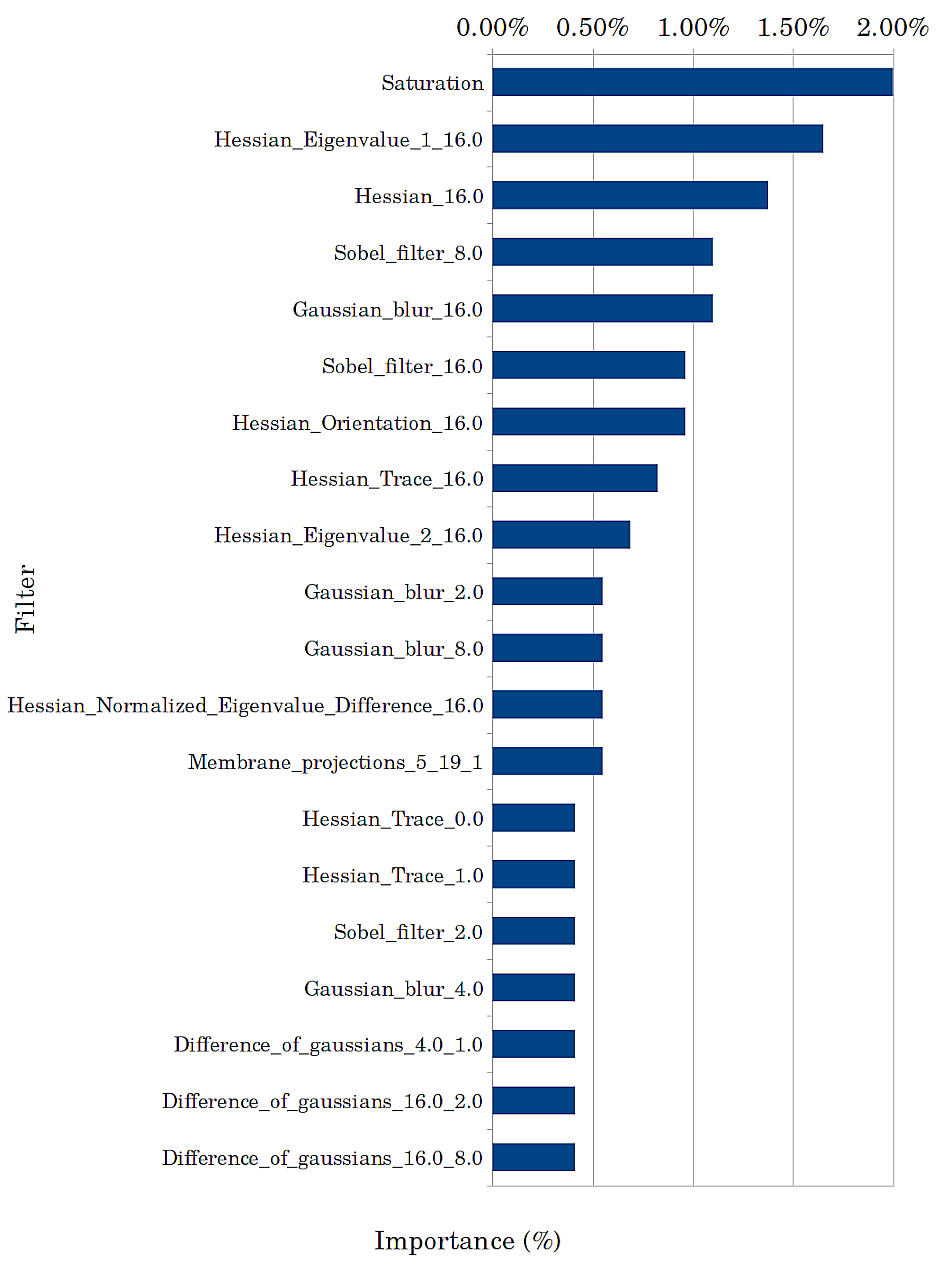
\includegraphics[width=1\linewidth]{gfx6/features/c1-importances} 
\caption[Feature importances test 1.]{Test 1: Feature importances results for classifier C1. This model used default settings. The feature stack for six slices with $ 79 $ features took $ 147138ms $ to create and the $ oo_b=1.98\%$. The highest ranking filters and respective importances are listed.}\label{fig:c1}
\end{figure}

\begin{figure}[!htbp]\myfloatalign
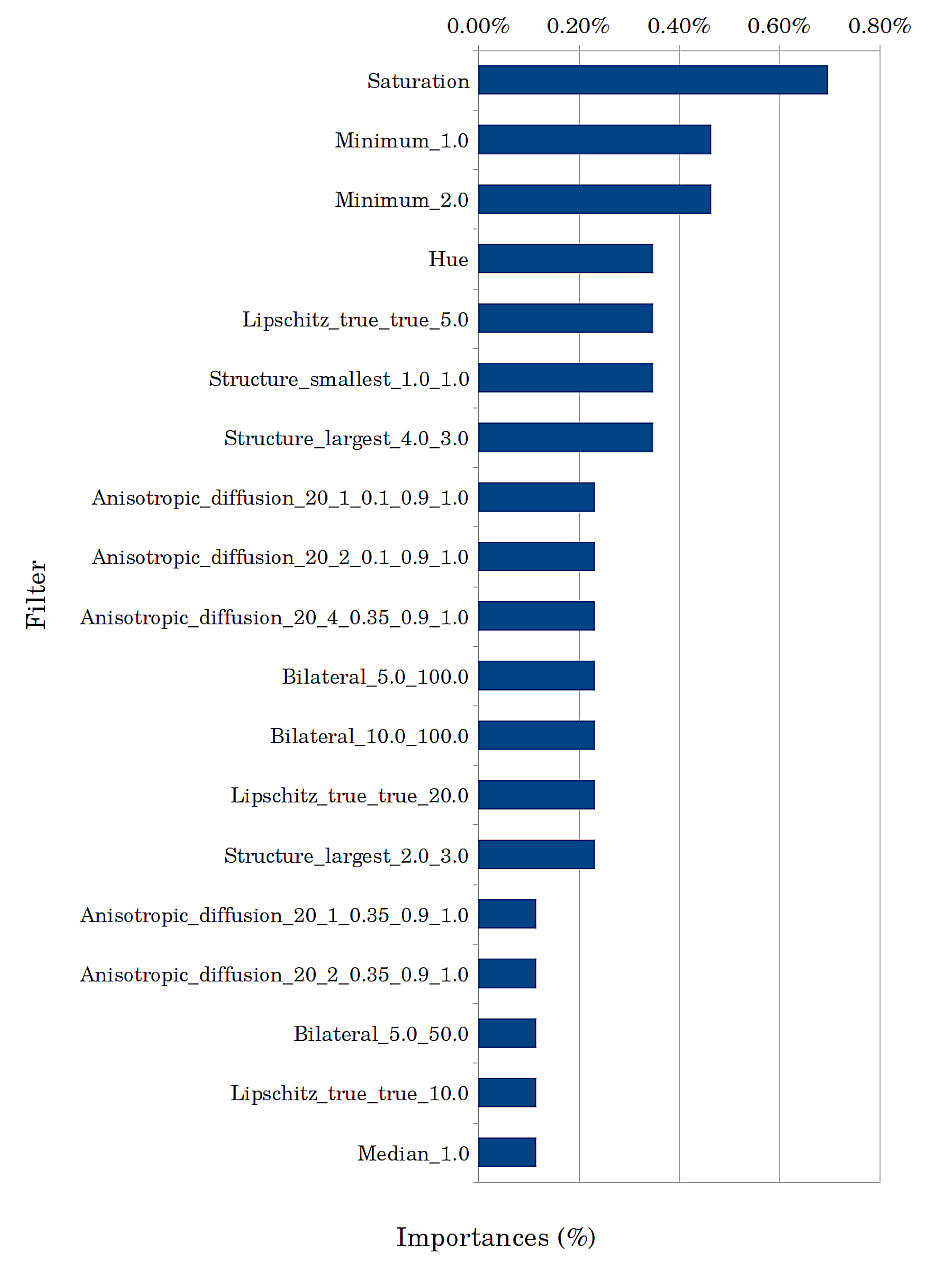
\includegraphics[width=1\linewidth]{gfx6/features/c2-importances} \caption[Feature importances classifier test 2.]{Test 2: Feature importance tests on classifier C2 which was optimised to produce the best segmentation of nest images. The feature stack for six slices with $ 46 $ features took $ 402974ms $ to create and the $ oo_b=0.93\% $. The highest ranking filters and respective importances are listed.}\label{fig:c2}
\end{figure}

\begin{figure}[!htbp]\myfloatalign
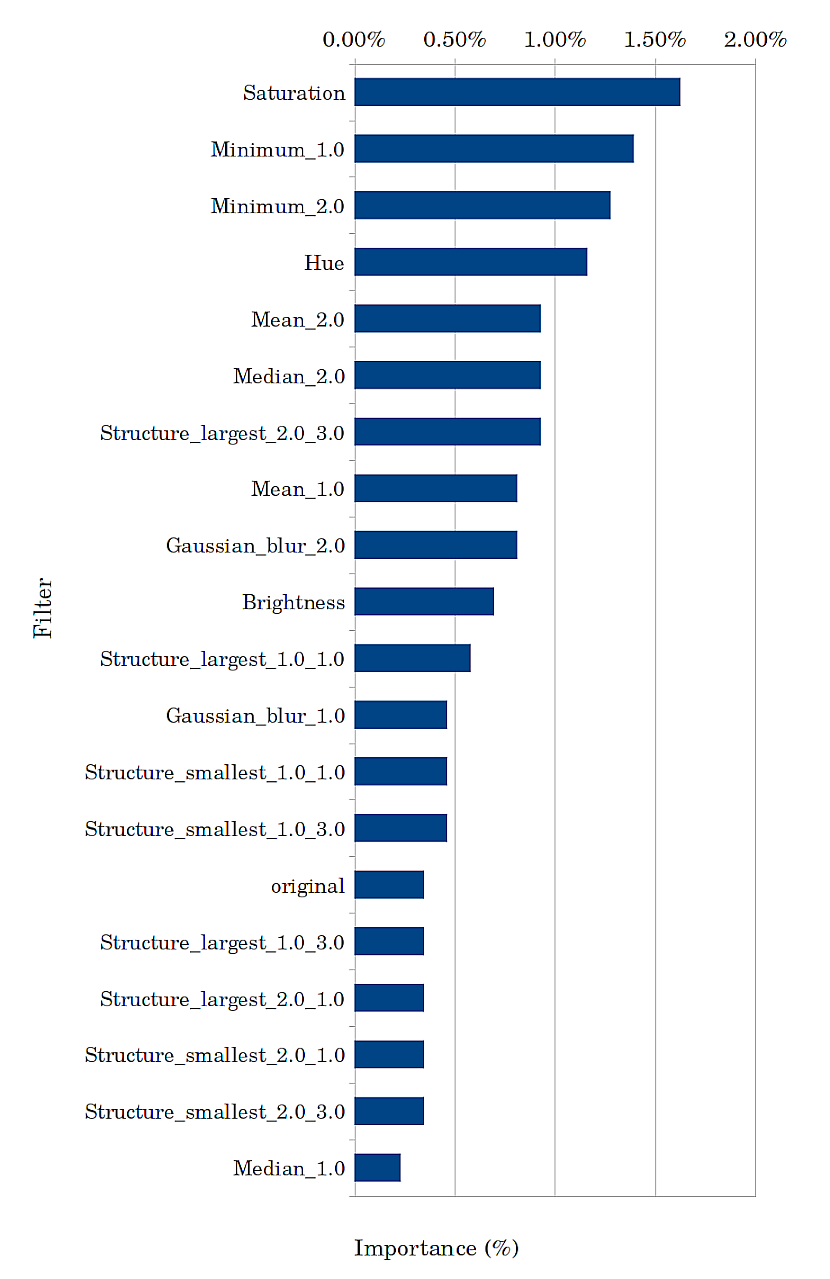
\includegraphics[width=1\linewidth]{gfx6/features/c3-importances} \caption[Feature importances classifier test 3.]{Test 3: Feature importance tests on classifier C3 which was optimised to speed up processing. The feature stack for six slices with $ 20 $ features took $ 23092ms $ to create and the $ oo_b=0.698\%$. All twenty filters were important and ranked as listed.}\label{fig:c3}
\end{figure}

\subsection{Number of trees}\label{sec:number-of-trees}
In Test 4, twenty two \ac{RF} models were loaded into Weka Experimenter \emph{Algorithms} in a 10 fold cross validation, 10 iteration test. The number of trees were adjusted $ N = 10 - 1000 $ in each of the 22 \ac{RF} models (shown along the bottom axis in Figure \ref{fig:trees}). Processing time exponentially increased with the number of trees. Performance gains did not appear significant beyond $N = 150$.

Classifier C4 was re-run via \ac{TWS} with $N = 50$, $ M = 2 $ and $ \sigma_{max} = 2 $. The \ac{TWS} settings for classifier C4 produced a features stack of 20. The number of pixels selected as $class_1 = 44$, $class_2 = 816$. The feature stack for six slices with $20$ features took $17503$ to create; and the $oo_b = 1.279\%$. The total model processing was around 12 x faster than C1; 32 x faster than C2 and 2 x faster than C3.

The $ oo_b $ from \ac{TWS} was different than reported in Weka Experimenter for the RF model with $N = 50$, $ M = 2 $ and $ \sigma_{max} = 2 $. Weka reported the $oo_b = 1.083\%$ (highlighted in orange on Figure \ref{fig:trees}). Tests were repeated using the rep\_nest.arff dataset. An alternative set-up was loaded. A 66.67\% split between training and tests (using randomised data) were applied in 500 iterations ($n = 500$). The error changed slightly to $oo_b = 1.151\%$; indicating the differences in $oo_b$ were most likely a consequence of the test configuration (i.e. evaluations run with a cross validation or \% data splits).

\subsection{Number of random features}\label{sec:number-of-random-features}
In Test 5, twenty \ac{RF} models were added to Algorithms for testing using a 10 fold cross validation experiment with 10 iterations. Each classifier model had a varying number of random features which were set between $M = 0-20$ (shown along the bottom axis on Figure \ref{fig:random-features}). 

Classifier C5 was re-run via \ac{TWS} with $N = 50$, $ M = 2 $ and $ \sigma_{max} = 8 $. The \ac{TWS} settings for classifier C5 produced a features stack of 20. The number of pixels selected as $class_1 = 44$, $class_2 = 816$. The feature stack for six slices with $20$ features took $17503ms$ to create; $oo_b = 0.628\%$. The total model processing was around 12 x faster than C1; 32 x faster than C2, 2 x faster than C3 and  was equal to C4.

The test results showed the performance improved when more random features were provided to the model for training and construction. The out of bag error for C5 ($oo_b = 0.628\%$) was lower than C5 ($oo_b = 1.279\%$). 

The final monitoring classifier (CF) used a \ac{RF} with $ F_{n} = 20 $, $ N = 50 $, $  M = 8 $ and $\sigma_{max} = 8 $ highlighted in orange on Figure \ref{fig:random-features}.

\begin{sidewaysfigure}[!htbp]\myfloatalign
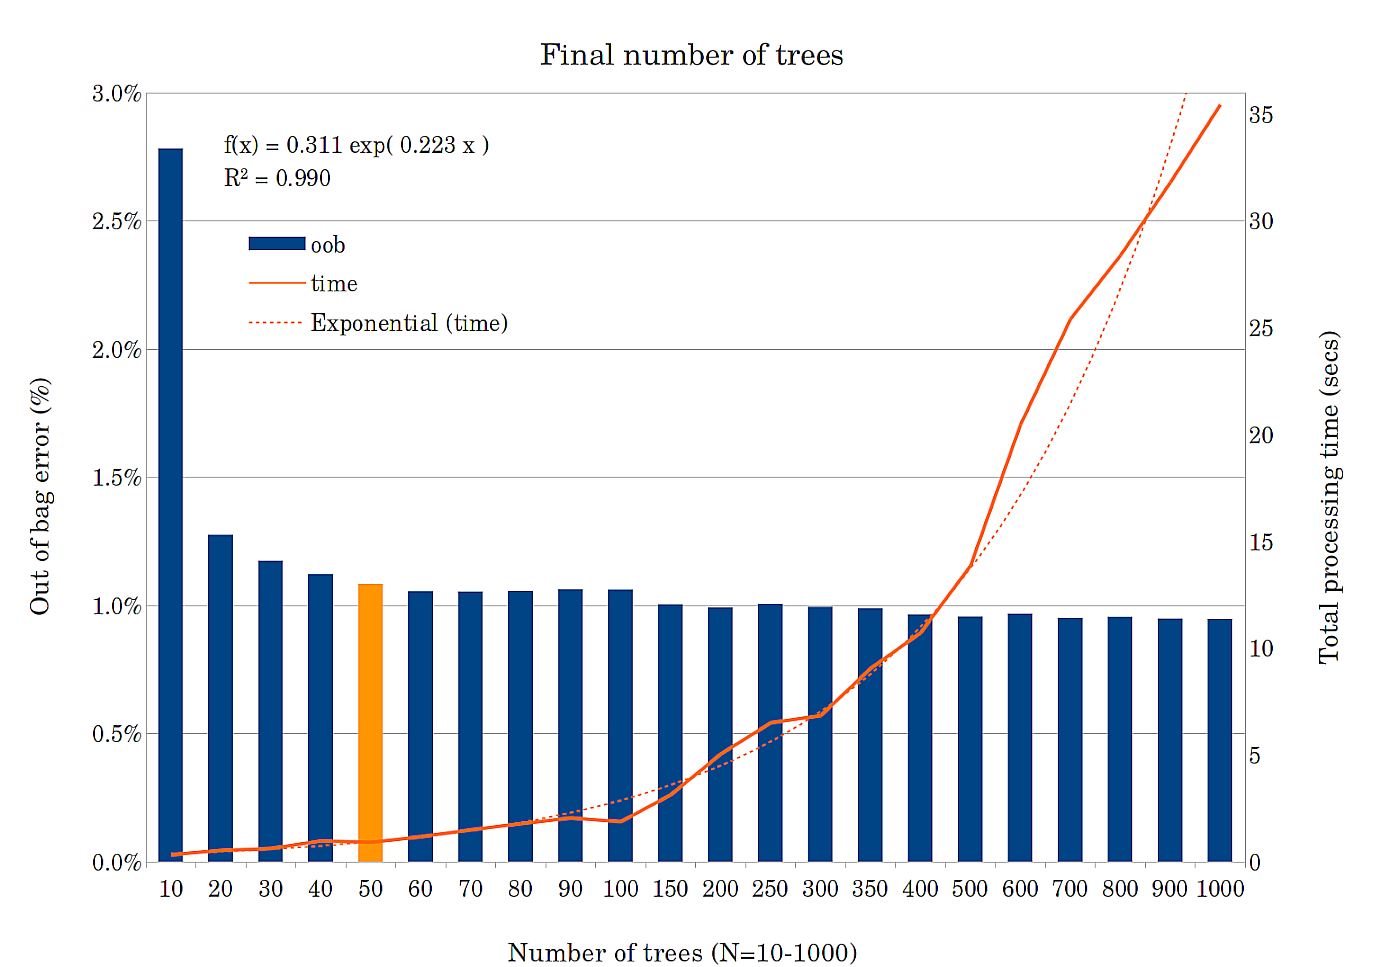
\includegraphics[width=0.9\linewidth]{gfx6/models/number-of-trees} \\
\caption[Number of trees.]{Test 4: \emph{Fifty trees ($ N = 50 $) were selected for the random forest model final monitoring classifier (CF). The out of bag error from Weka was $oo_b= 1.083\%$ (orange bar) and total processing time $ t_{total} = 0.925(sec)$ using the rep\_nest.arff dataset.}}\label{fig:trees}
\end{sidewaysfigure}

\begin{sidewaysfigure}[!htbp]\myfloatalign
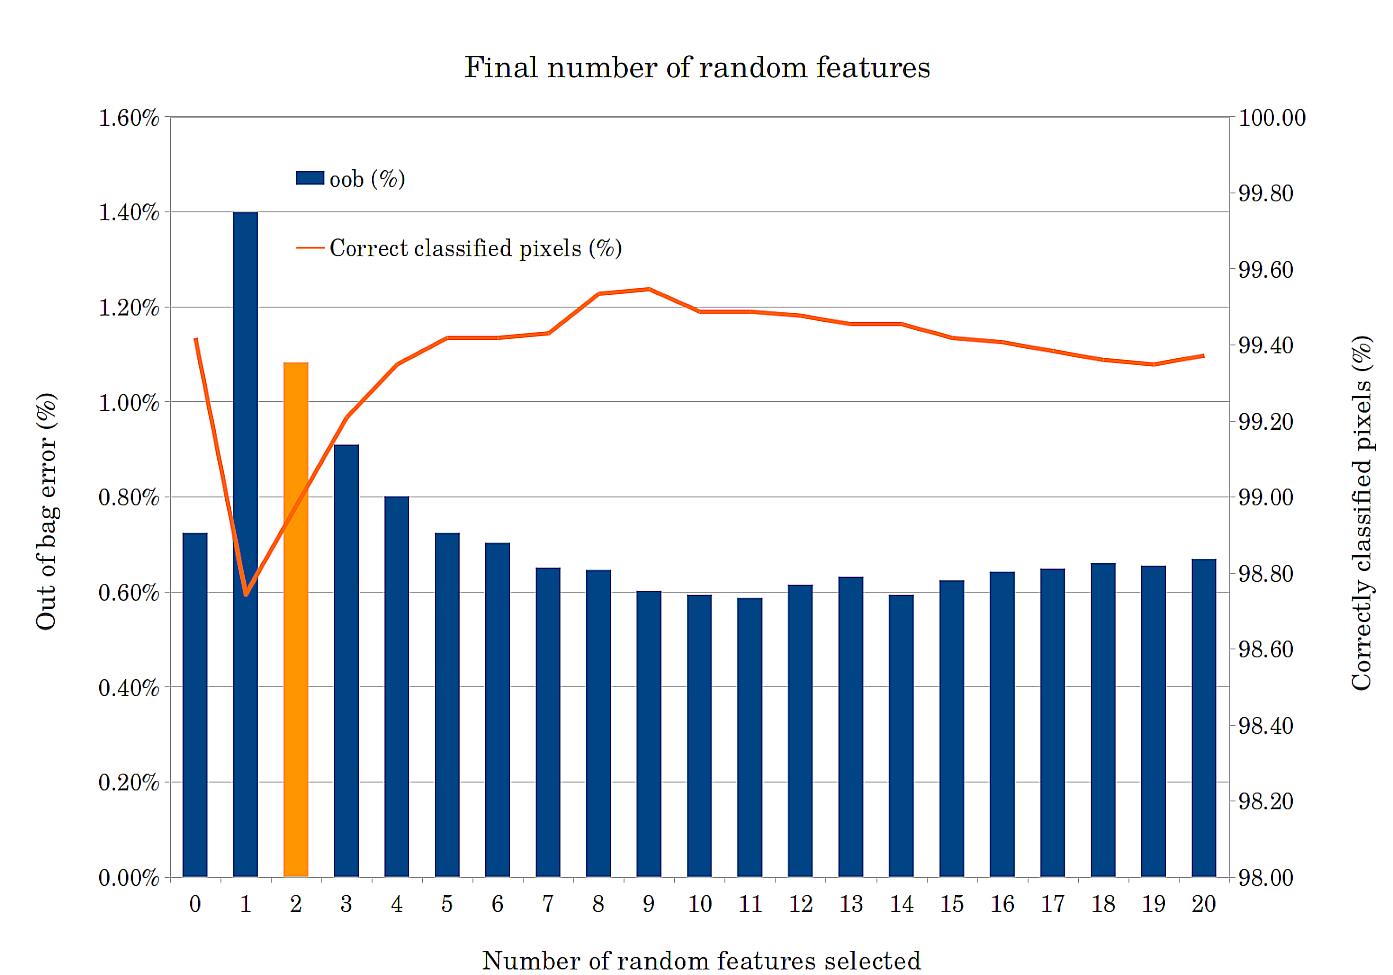
\includegraphics[width=0.9\linewidth]{gfx6/models/random-features} \\
\caption[Number of random features.]{Test 5: \emph{Two random features} ($ M = 8 $) were selected for the random forest model final monitoring classifier (CF). The out of bag error from Weka was $oo_b = 0.628\%$ (orange bar) and the percentage of correctly classified instances (pixels) $cc_{i} = 99.4\%$ using the rep\_nest.arff dataset.}\label{fig:random-features}
\end{sidewaysfigure}

\clearpage

\section{Classifier benchmarks}\label{sec:results-classifier-benchmarks}
The final test classifier CF was compared against nine machine learners. The results are listed in Table \ref{tab:benchmark} below. A 10 fold cross validation with 10 iterations was used in the experiment. The percentage of correctly classified instances were tested for $ n = 1000 $, with a confidence of 0.05 in a paired-corrected two tailed test. Results showed there were no signifiant improvements by any other models over CF; four gave results that were statistically worse. The naive Bayes model (M8) did not perform as well as CF on the test data-set with $ 90.35\% $ correct. The VotedPerceptron (M9, neural network) and SMO (M10, support vector machine) models also returned a lower number of correctly classified instances; $95.71\% $ and $96.74\%$ respectively. The ZeroR (M2) gave $ 94.88\%  $ correctly classified instances, slightly higher than naive Bayes model (M8).

\begin{table}[!htbp] \myfloatalign \caption[Classifier performance and benchmark results.]{Results of performance evaluations conducted in Weka experimenter. The final test classifier CF (M1) was benchmarked against nine other common models on the rep\_nest.arff dataset.\label{tab:benchmark}}
\begin{tabular}{llp{3.2in}} \toprule
Model & Correct (\%) & Weka model code\\ \midrule
M1 & 99.42 & hr.irb.fastRandomForest.FastRandomForest-I|50|-K|8|-S|1 \\ 
M2 & 94.88 $\bullet$ & rules.ZeroR  \\ \\
M3 & 98.37 & trees.J48-C 0.25 -M|2 \\ \\
M4 & 98.02 & trees.RandomTree-K|0|-M|1.0|-V|0.0010|-S|1 \\ \\
M5 & 99.19 & trees.RandomForest-I|10|-K|0|-S|1|-num-slots|1 \\ \\
M6 & 98.95 & hr.irb.fastRandomForest.FastRandomForest-I|50|-K|2|-S|1  \\
M7 & 99.07 & hr.irb.fastRandomForest.FastRandomForest-I|200|-K|2|-S|1 \\ 
M8 & 90.35 $\bullet$ & bayes.NaiveBayes  \\ \\
M9 & 95.71 $\bullet$ & functions.VotedPerceptron-I|1|-E 1.0|-S|1|-M|10000 \\ \\
M10 & 96.74 $\bullet$ & functions.SMO-C|1.0|-L|0.0010|-P|1.0E-12|-N|0|-V|-1|-W|1|-K|functions.supportVector.PolyKernel-E|1.0|-C|250007 \\ \\
\end{tabular} 
\begin{tabular}{c} \\
\small$\circ$, $\bullet$ statistically significant improvement or degradation\\ 
\end{tabular} 
\begin{tabular}{p{.3in}p{1in}p{3in}} 
& & \\ \bottomrule
\end{tabular} 
\end{table} 

\section{Segmentation performance}\label{sec:segmentation-performance}
The representative image stack of six images were fully processed using the final test classifier (CF). A trace was added and the model was re-trained (CF2). Another trace ws added and the model was trained again (CF3). The complete processing pipeline is shown in Figure \ref{fig:test-stack-processed}.

The out of bag error decreased slightly to $ oo_b= 0.98\%$ when the second trace was included in training (CF3). The final counts were visually checked against raw \ac{RGB} images for verification and against the manual field counts as detailed in Table \ref{tab:test-classifier-results} below. Classical threshold methods were tested. Intensity, statistical region merging and canny edge detectors were operations were applied to the test stack. 

\begin{table}[!htbp]\myfloatalign \caption[Final count results from test classifier CF.]{The final automatic count results  on representative images (slices 1--6) using CF$ _{rt} $ compared to classical segmentation methods, manual-image and manual-field counts.}\label{tab:test-classifier-results} 
\begin{tabular}{lllllll} \toprule
Method &	s1 &	s2 &	s3 &	s4 &	s5 &	s6 \\ \toprule
Manual image &	3 &	3 &	3 &	2 &	2 &	2   \\
Manual field &	2 &	4 &	4 &	3 &	4 &	9 \\
CF1 &	21 &	11 &	14 &	22 &	4 &	64  \\
CF2 &	21 &	2 &	3 &	13 &	3 &	14  \\
CF3 &	7 &	1 &	8 &	4 &	2 &	3 \\
Haung4 &	87 &	89 &	51 &	50 &	51 &	62  \\
Mean5 &	87 &	89 &	51 &	50 &	51 &	62  \\
MinError6 &	87 &	89 &	51 &	50 &	51 &	62  \\
Min7 &	87 &	89 &	51 &	50 &	51 &	62  \\
Otsu8 &	87 &	89 &	51 &	50 &	51 &	62  \\
Srm9 &	4 &	3 &	2 &	2 &	5 &	5  \\
Srm10 &	1 &	2 &	0 &	0 &	2 &	2  \\
Srm11 &	1 &	2 &	1 &	1 &	1 &	1 \\
Srm12 &	41 &	57 &	10 &	28 &	99 &	14  \\
Srm13 &	60 &	72 &	24 &	42 &	114 &	20  \\
Cedge14 &	93 &	62 &	41 &	70 &	95 &	25  \\
Cedge15 &	88 &	92 &	48 &	62 &	39 &	10  \\
Cedge16 &	170 &	202 &	71 &	91 &	133 &	20  \\
Cedge17 &	191 &	230 &	63 &	99 &	149 &	22  \\
Cedge18 &	179 &	225 &	49 &	96 &	169 &	19  \\
Cedge19 &	175 &	225 &	64 &	103 &	143 &	22  \\
Cedge20 &	189 &	226 &	46 &	103 &	179 &	16  \\
\bottomrule
\end{tabular}
\end{table}

\begin{figure}[!htbp]\myfloatalign
\subfloat[Raw stack imges.]{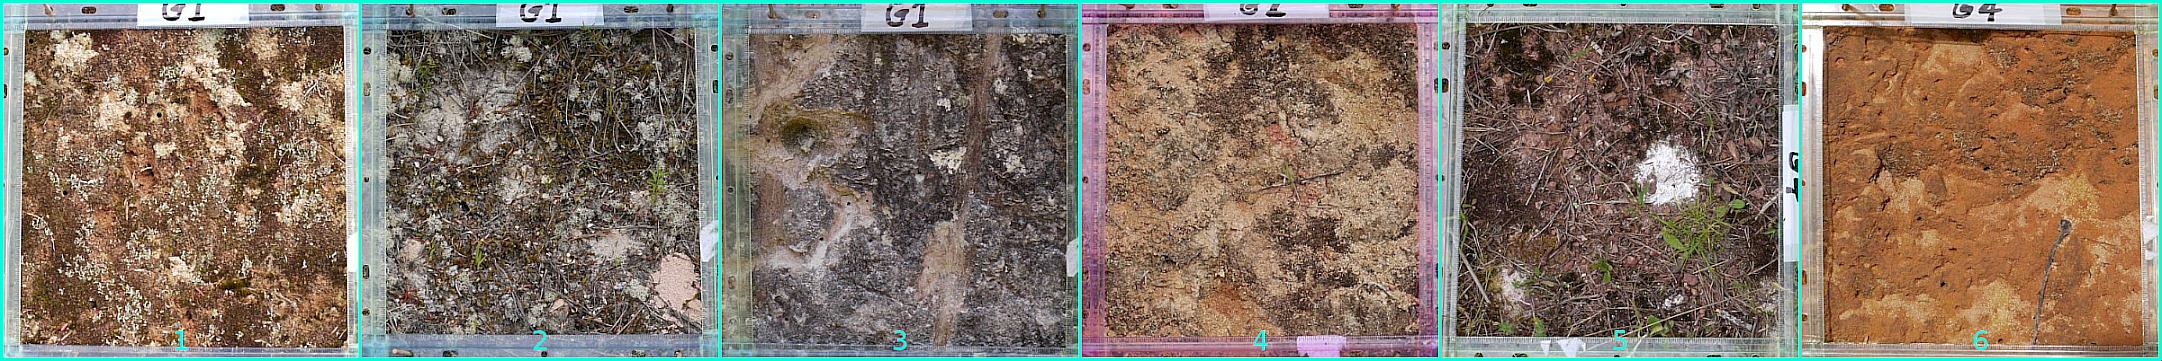
\includegraphics[width=1\linewidth]{gfx6/segtest/1rf}} \\
\subfloat[Classified outputs.]{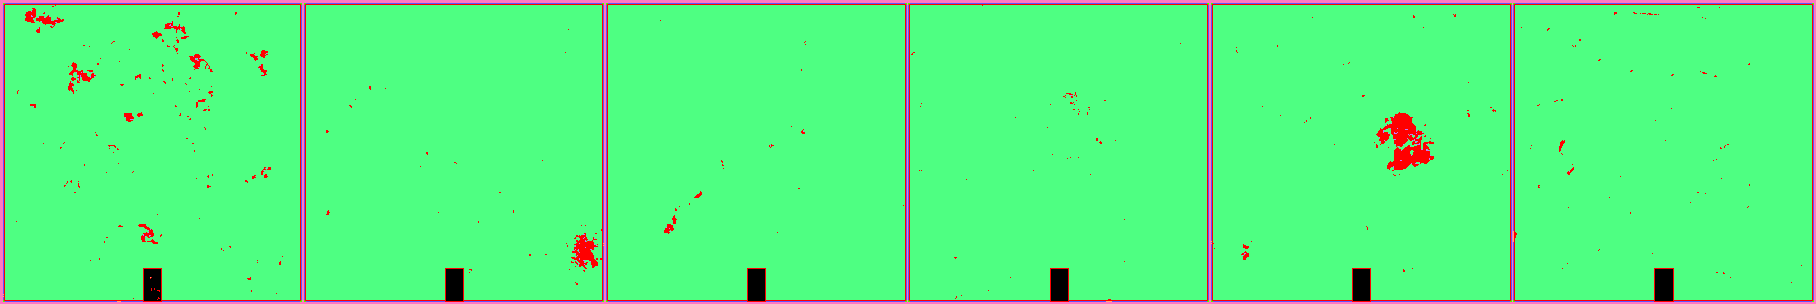
\includegraphics[width=1\linewidth]{gfx6/segtest/2rf}} \\
\subfloat[Converted to 8-bit binary. ]{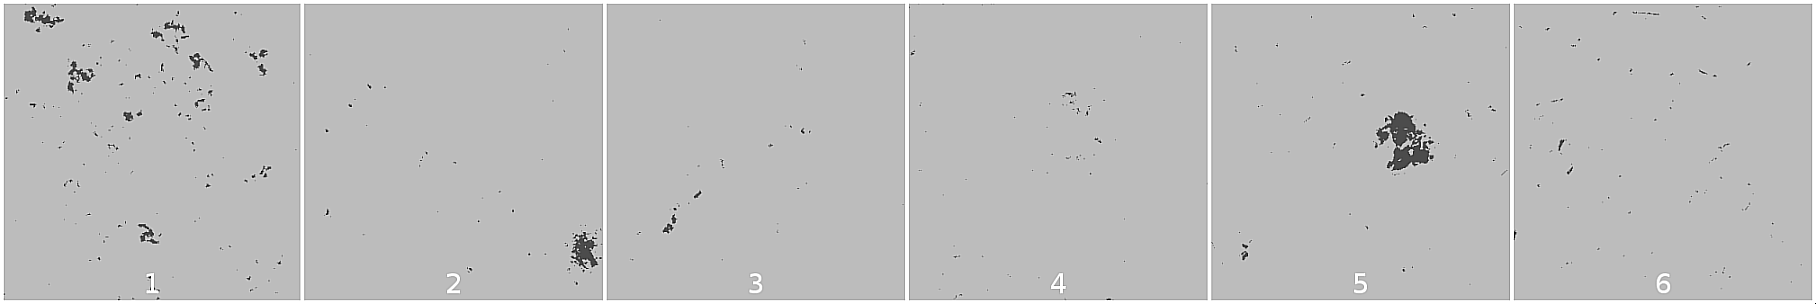
\includegraphics[width=1\linewidth]{gfx6/segtest/3rf}} \\
\subfloat[Binary oprators applied.]{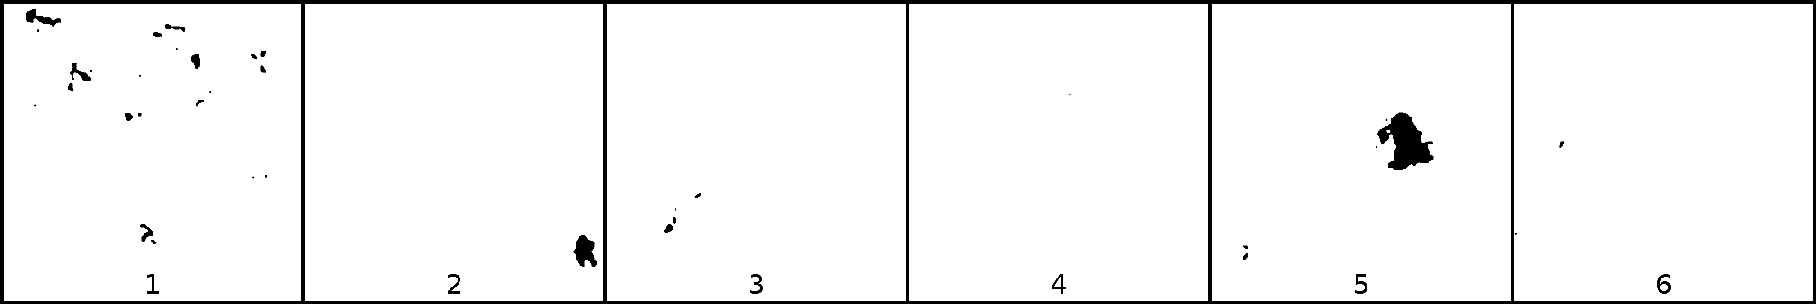
\includegraphics[width=1\linewidth]{gfx6/segtest/4rf}} \\
\subfloat[Particle Anlysis.]{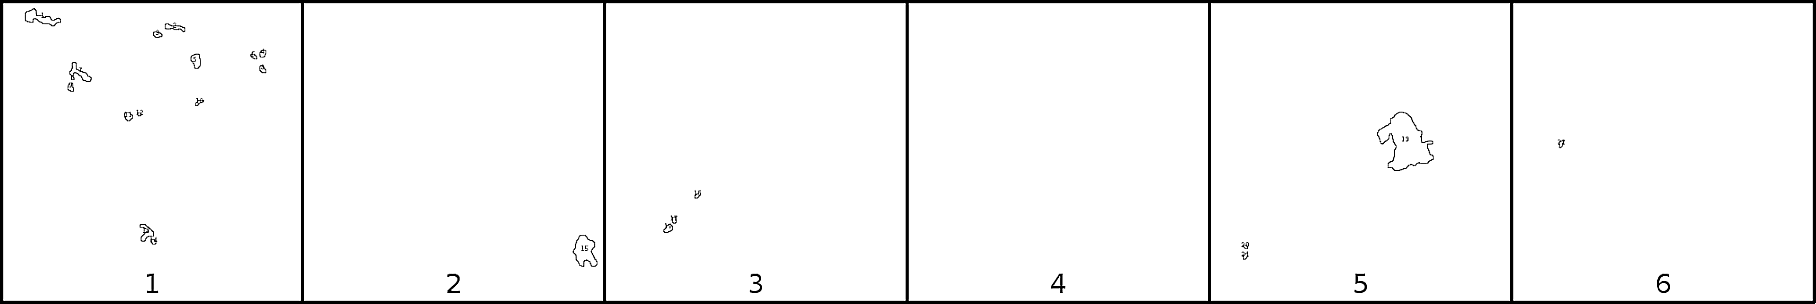
\includegraphics[width=1\linewidth]{gfx6/segtest/5rf}} \\
\caption[Test image stack.]{Representative images in (a) the test stack used to train initial classifiers (C1--C5). The classified results from CF{\scriptsize re-trained} (b) were post-processed (c)-(d) to give the (e) final counts. These were compared against classical segmentation methods, visual nest counts from images, and the manual counts taken in the field.}\label{fig:test-stack-processed}
\end{figure}

\section{Training stacks}\label{sec:training-stacks}
The four training stacks collated for each site are displayed in the Figures \ref{fig:train-t1}, \ref{fig:train-p2}, and \ref{fig:train-m3} below. They demonstrate the wide variation in images between and within monitoring sites. All the trainings stacks contained an image of the control grid, (e.g. slice 2 for Mt. Tiger and Mt. Parihaka, and slice 1 for Memorial Drive) and the images of inactive nests acquired May 21 2013. Slices were arranged in date sequence. These were used for classifier training; final classifiers were applied to all monitoring stacks.

\begin{sidewaysfigure}[!htbp]\myfloatalign
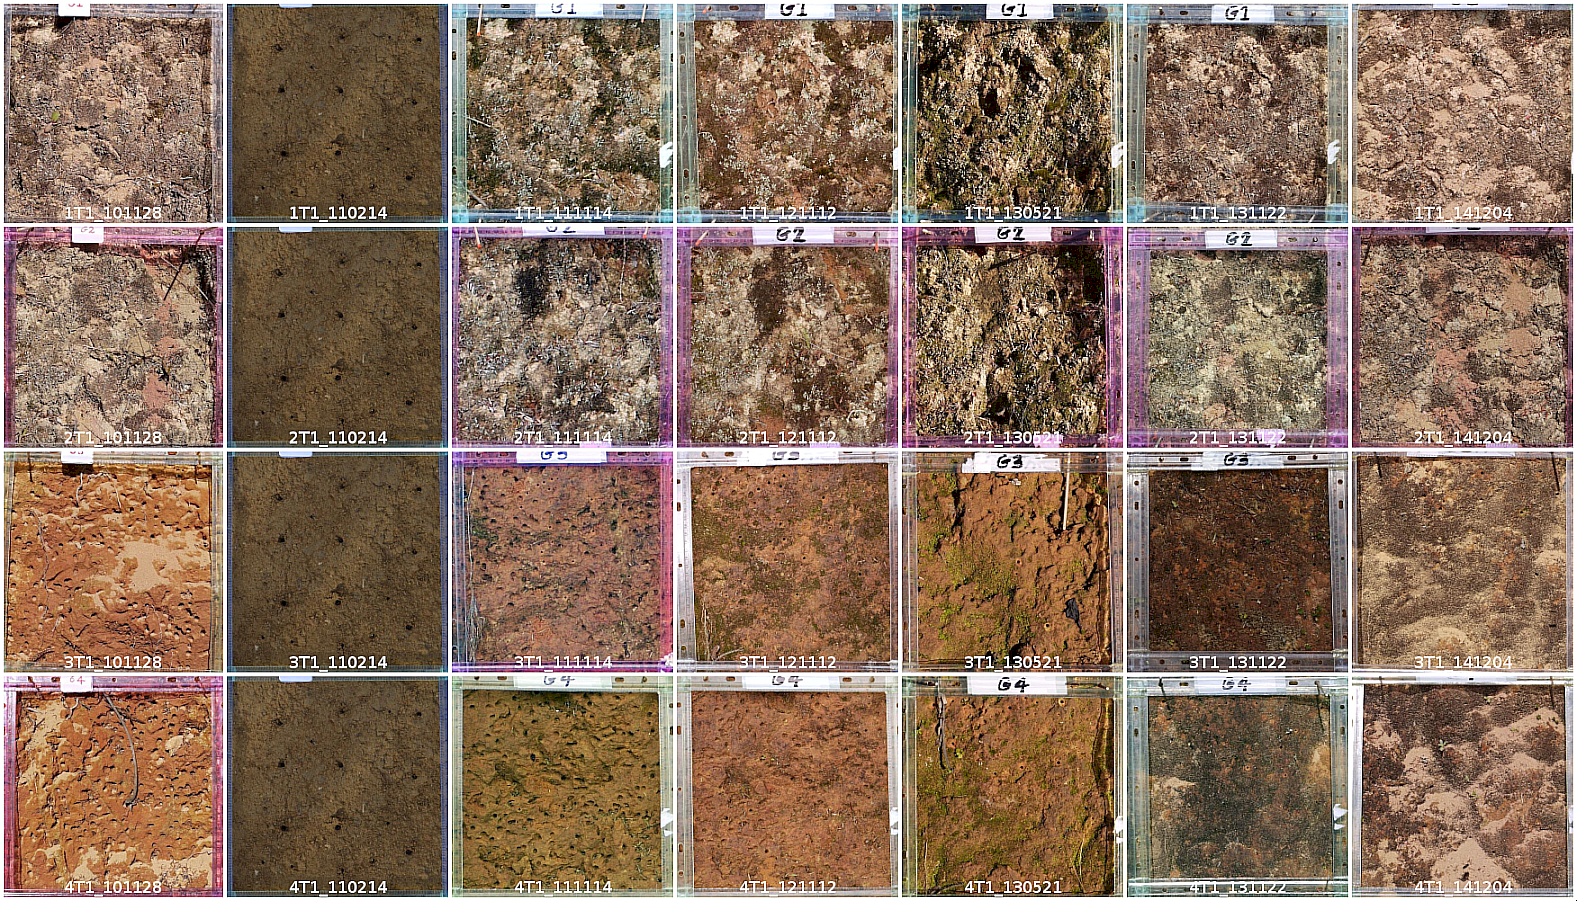
\includegraphics[width=1\linewidth]{gfx6/train/train-t1} \\
\caption[Site 1: training stacks for Mt. Tiger. ]{Site 1: Training stacks for Mt. Tiger. Slices of collection years from left to right and grid numbers 1--4, from top to bottom. Slice 1 = control and slice 4 = inactive nest. All nests were on a roadside bank with an approximate slope ranging between 60--80\textdegree. There were no horizontal ground nests at this location. Images from grids 1--2 and grids 3--4 were similar in appearance.}\label{fig:train-t1}
\end{sidewaysfigure}

\begin{sidewaysfigure}[!htbp]\myfloatalign
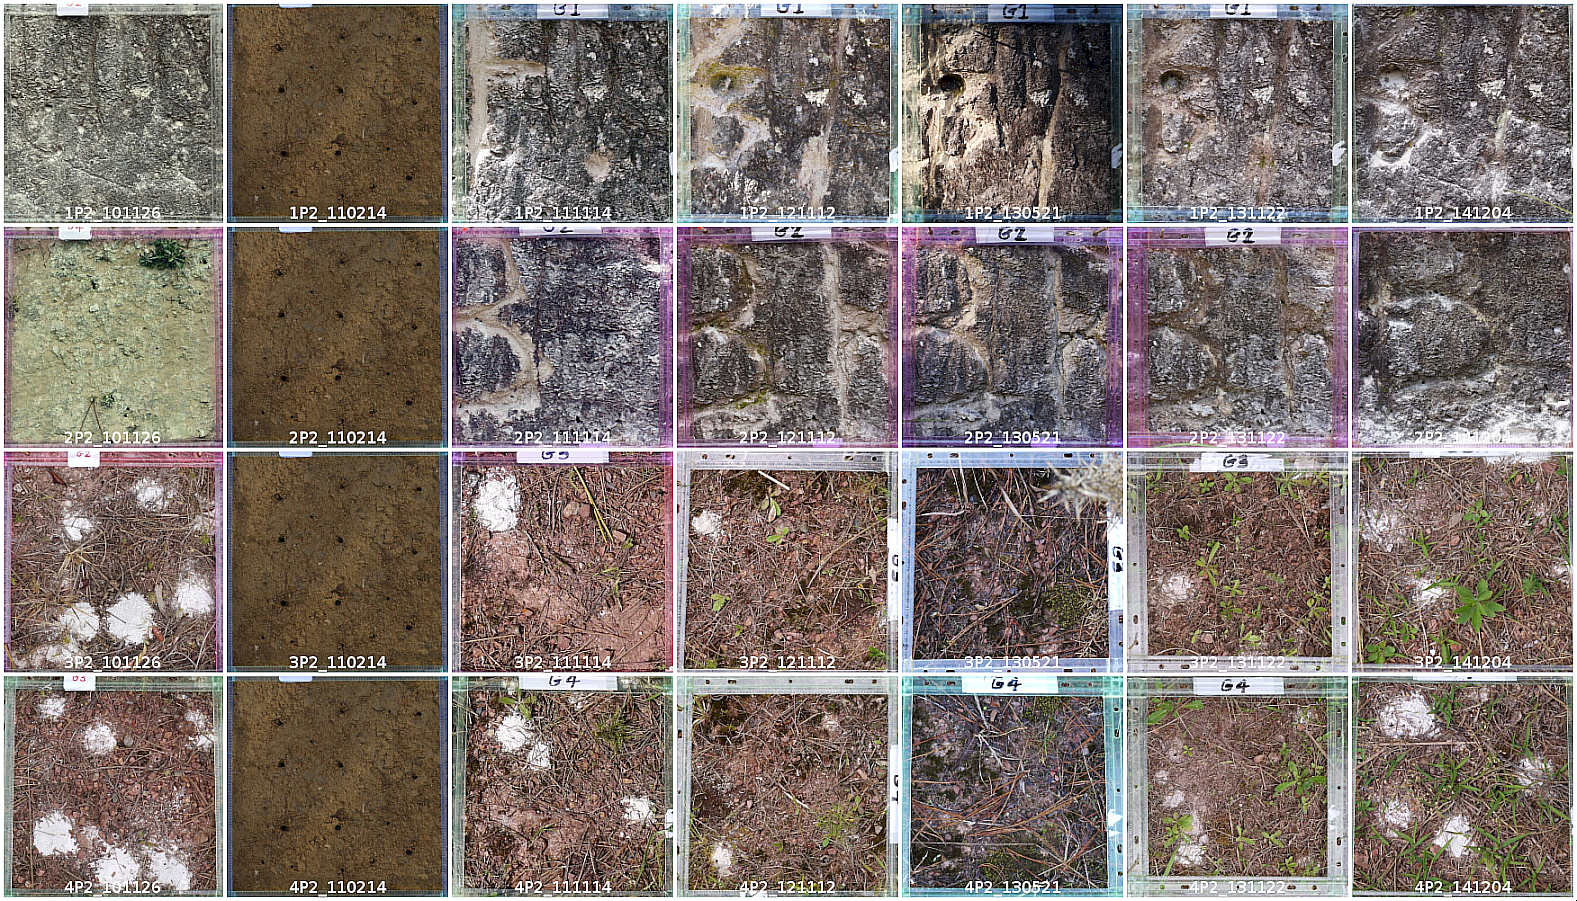
\includegraphics[width=1\linewidth]{gfx6/train/train-p2} \\
\caption[Site 2: training stacks for Mt. Parihaka.]{Site 2: training stacks for Mt. Parihaka. Slices of collection years from left to right and grid numbers 1--4, from top to bottom. Slice 1 = control and slice 4 = inactive nest. The nests in grids 1--2 were on a large bank (~5m long x 8m high) with an approximate slope ranging between 60--80\textdegree; grids 3--4 were horizontal ground nests. Images from grids 1--2 and grids 3--4 were similar in appearance.}\label{fig:train-p2}
\end{sidewaysfigure}

\begin{sidewaysfigure}[!htbp]\myfloatalign
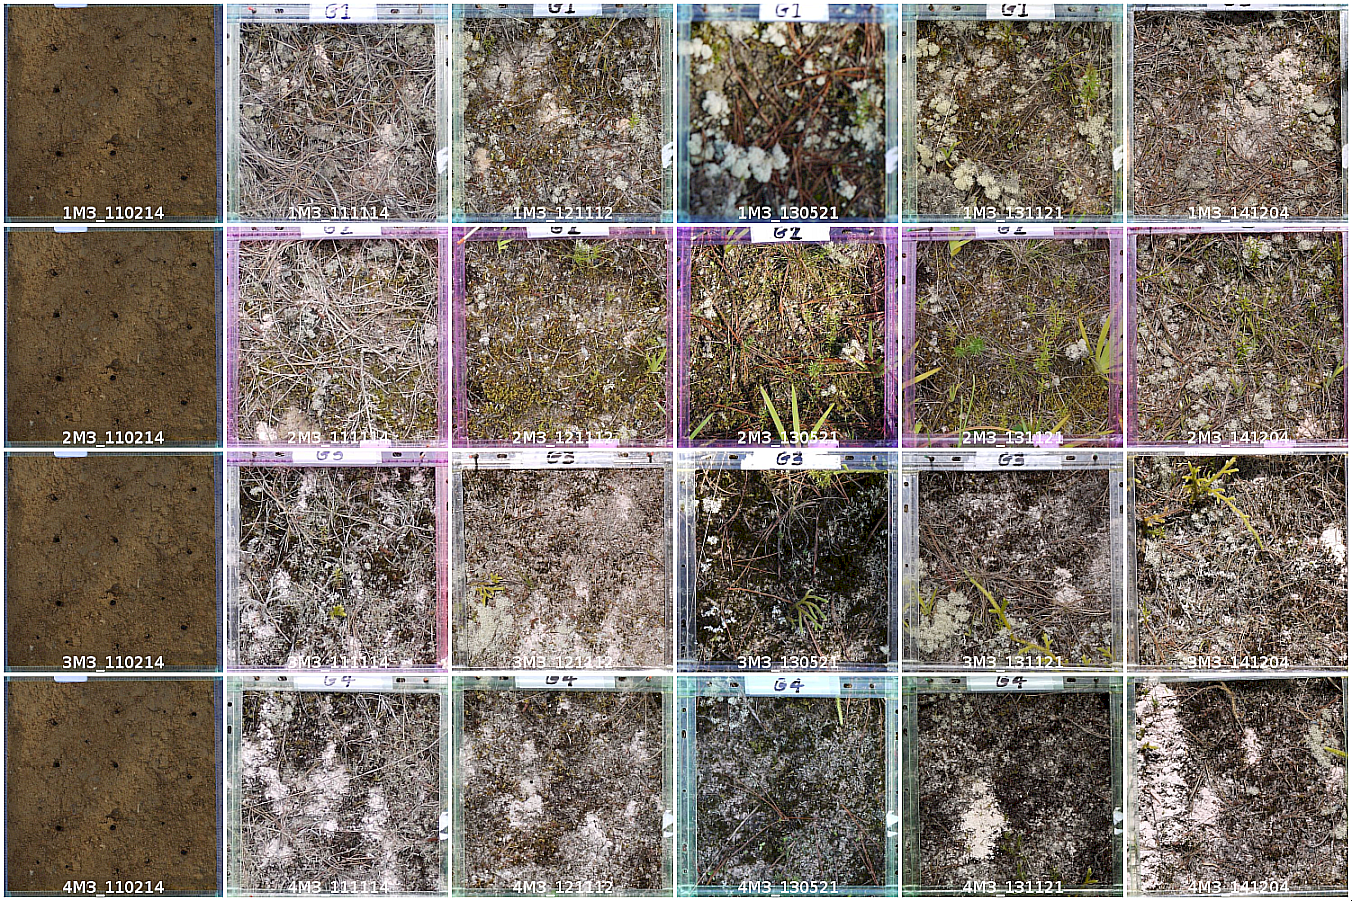
\includegraphics[width=1\linewidth]{gfx6/train/train-m3} \\
\caption[Training stack Memorial Drive.]{Training stack Memorial Drive. Slices of collection years from left to right and grid numbers 1--4, from top to bottom. Slice 2 = control and slice 5 = inactive nest. All nests were on a roadside bank with an approximate slope ranging between 60--80\textdegree. There were no horizontal ground nests at this location. All grid images were similar in appearance.}\label{fig:train-m3}
\end{sidewaysfigure}

\section{Monitoring data summary}\label{sec:monitoring-data-summary}
A summary of collections are shown in the next few sections including a statistical summary of data, and preliminary distribution evaluations. Once the CF classifiers were trained, processing (classifications and post-processing) was completed in less than 24 hours. Field monitoring was conducted in a single two and half hour round trip, beginning at site 1 and ending at site 3. The time to conduct manual nests counts was approximately 15 minutes per site. The time taken to acquire images was around 5 minutes per site.

\subsection{Collections}\label{sec:collections}
A total of 158 monitoring days resulted in 632 images per image collection. Around 1/3 of image data were unrecoverable (612 images). A summary of collections over five years (2010--2014) for Mt. Tiger, Mt. Parihaka and Memorial Drive are shown Table \ref{tab:collections-summary} below.

\begin{table}[!htbp] \myfloatalign \caption[Field collection summary of monitoring days.]{Field collection summary of monitoring days for three locations, Mt. Tiger (S1), Mt. Parihaka (S2) and Memorial Drive (S3) over five years (2010--2014)}\label{tab:collections-summary} 
\begin{tabular}{llllllp{0.9in}} \toprule
Site ID& 2010 & 2011 & 2012 & 2013 & 2014 & Total days \\ \midrule
S1 & 16 & 16 & 13 & 10 & 3 & 59 \\
S2 & 16 & 16 & 13 & 10 & 3 & 59 \\
S3 & ND & 16 & 13 & 10 & 3 & 43 \\
Yearly totals & 32 & 48 & 39 & 30 & 9 & 158 \\ \bottomrule
\end{tabular}
\begin{tabular}{l}\\
\textasteriskcentered Total processed images = 1896 \\
\textasteriskcentered Monitoring images = 1284 \\ 
\textasteriskcentered Field samples = 632 \\ 
\end{tabular}
\end{table}

\subsection{Descriptive statistics}\label{sec:descriptive-statistics}
The mean, standard deviation and variances for manual field and automatic counts are shown in Table \ref{tab:descriptive-statistics-summary} below. The variances were larger than the means for both methods and the dispersal index suggests clustering; data fits a negative binomial model.

\begin{table}[!htbp] \myfloatalign \caption[Descriptive statistics summary.]{Descriptive statistics summary.}\label{tab:descriptive-statistics-summary} 
\begin{tabular}{p{0.6in}p{0.4in}p{0.4in}p{0.4in}p{0.4in}p{0.4in}p{0.4in}p{0.4in}} \toprule
Method & n	& $ \mu $& $ SE $ & $\sigma $	& SD & DI & CV \\ \midrule
Automatic & 	1284 & 	6.424 & 	0.284 & 	103 & 	10 & 	16 & 	1.58 \\
Manual &	1896 & 	4.545 & 	0.136 & 	35 & 	5 & 	7 & 	1.31 \\ 
 \bottomrule
\end{tabular} 
\begin{tabular}{p{3.4in}llll} \\
\emph{Table key }& & & & \\
Sample & & & &  $ n $\\
Mean & & & &  $ \mu $\\
Standard error of the mean ($ SD/\sqrt{n} $) & & & & $SE$ \\
Variance & & & &  $\sigma $ \\
Standard deviation & & & &  SD \\
Dispersal index ($ \sigma/mean $) & & & &  DI \\
Coefficient of variation ($ SD/mean $) & & & & CV \\ 
\end{tabular}
\end{table}

\subsection{Frequency distribution}\label{sec:frequency-distribution}
The frequency distribution of automatic and manual field nest counts using observed and expected values are shown in Figure \ref{fig:binomial}. The observed data agrees with the expected frequency distribution of a negative binomial model for the automatic method. The observed and predicted frequency distribution for the manual method does not show the same strength of agreement with a negative binomial model. 

\begin{sidewaysfigure}[!htbp]
\myfloatalign
{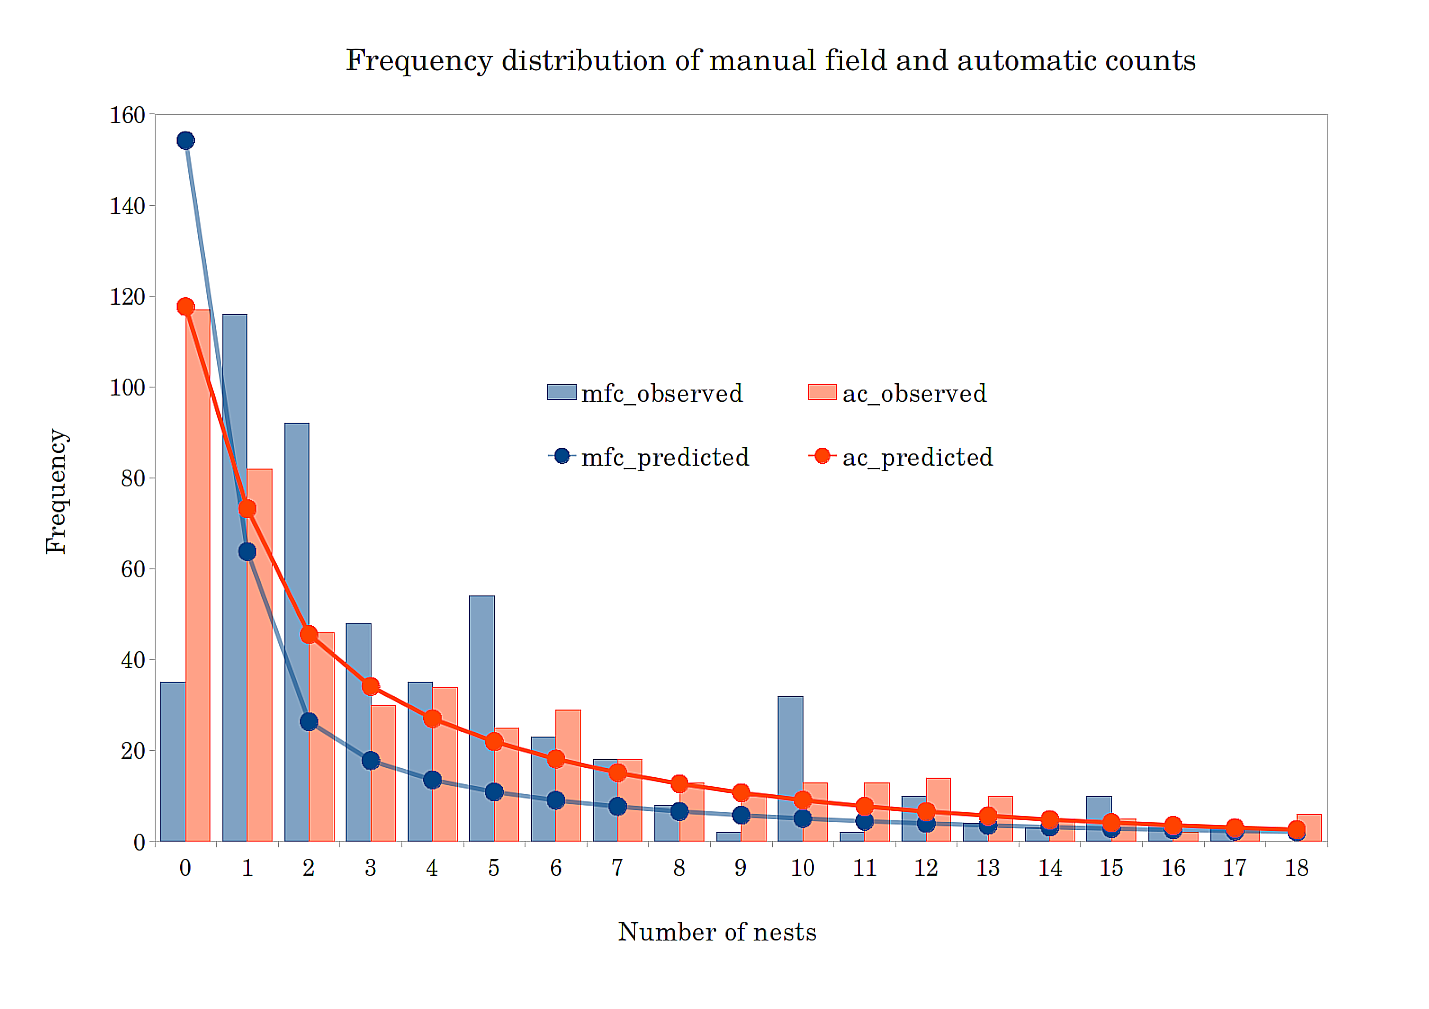
\includegraphics[width=0.9\linewidth]{gfx6/results/binomial}}
\caption [Frequency distribution of nest counts.]{Frequency distribution of automatic (ac in red) and manual field (mfc in blue) nest counts. Histograms show the observed frequency distributions for manual field counts and automatic counts. Matching coloured lines, joined with close circles are the predicted frequencies expected from a negative binomial model.} \label{fig:binomial}
\end{sidewaysfigure}
\clearpage

\section{Number of active nests by method}\label{sec:number-of-active-nests-by-method}

Lin's concordance of correlation was used to compare methods by measuring the precision ($ r $), agreement ($\rho_{c}$) and accuracy ($C_{b}$); data were calculated using the epi.ccc function within the epiR package. Plots were generated in epiR to display the line of perfect concordance (dashed) and the  line of best fit (solid) for each analysis (1--5) which are outlined  and summarised in Table \ref{tab:counts-by-different-methods}. 

\begin{table}[!htbp]\myfloatalign
\caption[Summary of comparative analyses.]{Five comparative analyses and a summary of the most important descriptive parameters used to measure precision ($r$), agreement ($\rho_{c}$) and accuracy ($C_{b}$) between methods.}\label{tab:counts-by-different-methods}
\begin{tabular}{p{0.4in}p{0.9in}p{0.9in}p{0.3in}p{0.3in}p{0.3in}p{0.3in}} \toprule
Analysis & Method 1 & Method 2 & $ n $ & $r$ & $\rho_{c}$ & $C_{b}$ \\ \midrule
A1 & a-ths & a-CF & 1284 & 0.244 & 0.040 & 0.164 \\
A2 & m-image ob1 & m-image ob2 & 170 & 0.891 & 0.867 & 0.973 \\
A3 & m-field & m-image & 170 & 0.641 & 0.622 & 0.97 \\
A4 & m-image & a-CF & 170 & 0.705  &  0.679 & 0.963 \\
A5 & m-field & a-CF & 520 &  0.828  & 0.738 & 0.891 \\ \bottomrule
\end{tabular} 
\begin{tabular}{p{3.6in}l} \\
\emph{Table key} & \\ 
Automatic (a-) and manual (m-) methods &\\
Images segmented by monitoring classifier CF  &  a-CF \\
Images segmented by default thresholds & a-ths\\
Nests counted from images by two scorers  & ob1-2 \\
Number of (paired) samples &  $ n $\\
Pearson's correlation coefficient (precision)&  $r$ \\
Lin's Concordance of Correlation (agreement) &  $ \rho_c $ \\
Bias correction factor (accuracy)  $ = \rho_c/r $ & $ C_{b} $ \\
\end{tabular}
\end{table}

\subsection{Classical threshold and machine learner}\label{sec:classical-threshold-and-machine-learner}

An evaluation of nest counts derived from thresholding and CF model segmentations are shown in Figure \ref{fig:automatic-thresh-c4}. The methods show poor agreement ($\rho_{c} = 0.040$) and accuracy ($C_{b} = 0.164$); with a very weak positive correlation ($r = 0.214$, $P < 0.05 $).

\begin{figure}[!htbp]\myfloatalign
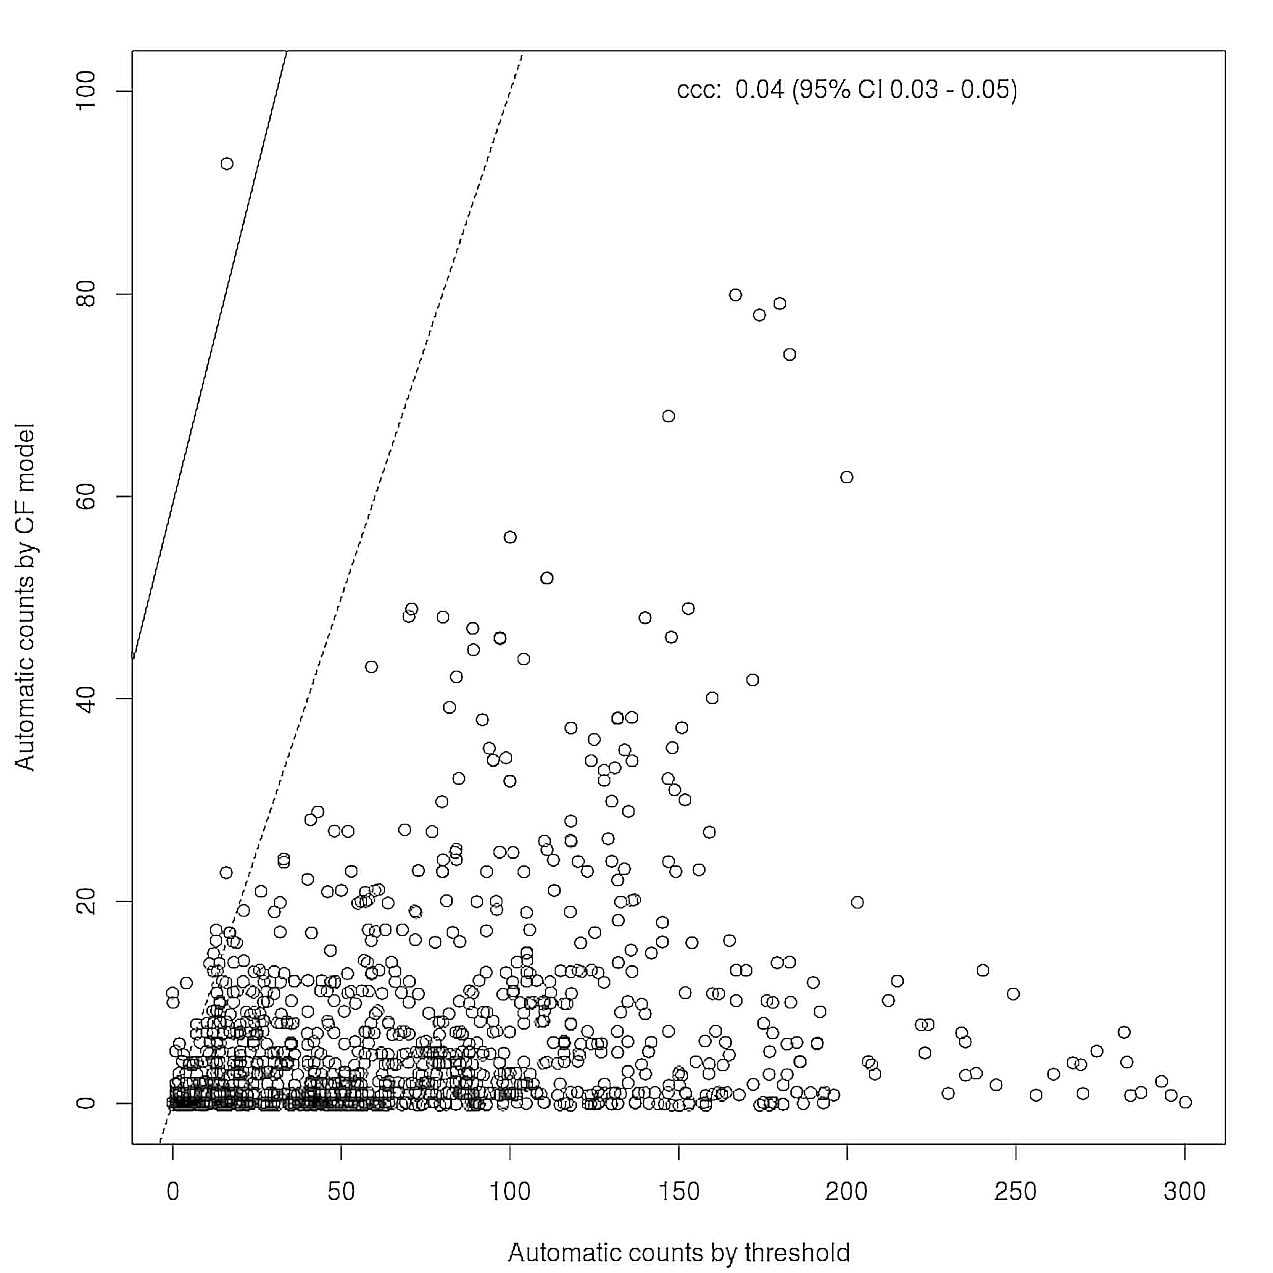
\includegraphics[width=1\linewidth]{gfx6/results/a1} \\
\caption[Automatic counts by threshold and model CF.]{Analysis 1: A comparison of nest counts by different image analysis methods. Automatic counts from monitoring image stacks using classical thresholding (default intensity histogram) and the CF model (RF classifier). The dashed line shows perfect concordance; the solid line is the line of best fit. Performance measures: $r = 0.244$ (precision), $\rho_{c} = 0.040$ (agreement) and $C_{b} = 0.164$ (accuracy).}\label{fig:automatic-thresh-c4}
\end{figure}

\clearpage

\subsection{Manual-field and image counts}\label{sec:manual-field-and-image-counts}
Manual nest counts estimated from images and actual numbers taken in the field were compared. The variability between two image counts by two scorers are outlined first. Nest counts estimated from images by two scorers were compared to analyse the variability between observers. Figure \ref{fig:manual-image-ob1-ob2-alldata} shows the output results from epiR. There was close agreement between the estimates from two scorers ($\rho_{c} = 0.867$) with good precision ($r = 0.891$) and accuracy ($C_{b} = 0.973$). The mean estimated counts for two scorers ($ n = 170 $) were compared against manual field counts in Figure \ref{fig:manual-feild-manual-image}. There was close agreement between the counts from two methods ($\rho_{c} = 0.622$), good precision ($r = 0.641$) and accuracy ($C_{b} = 0.97$).

\begin{figure}[!htbp]\myfloatalign
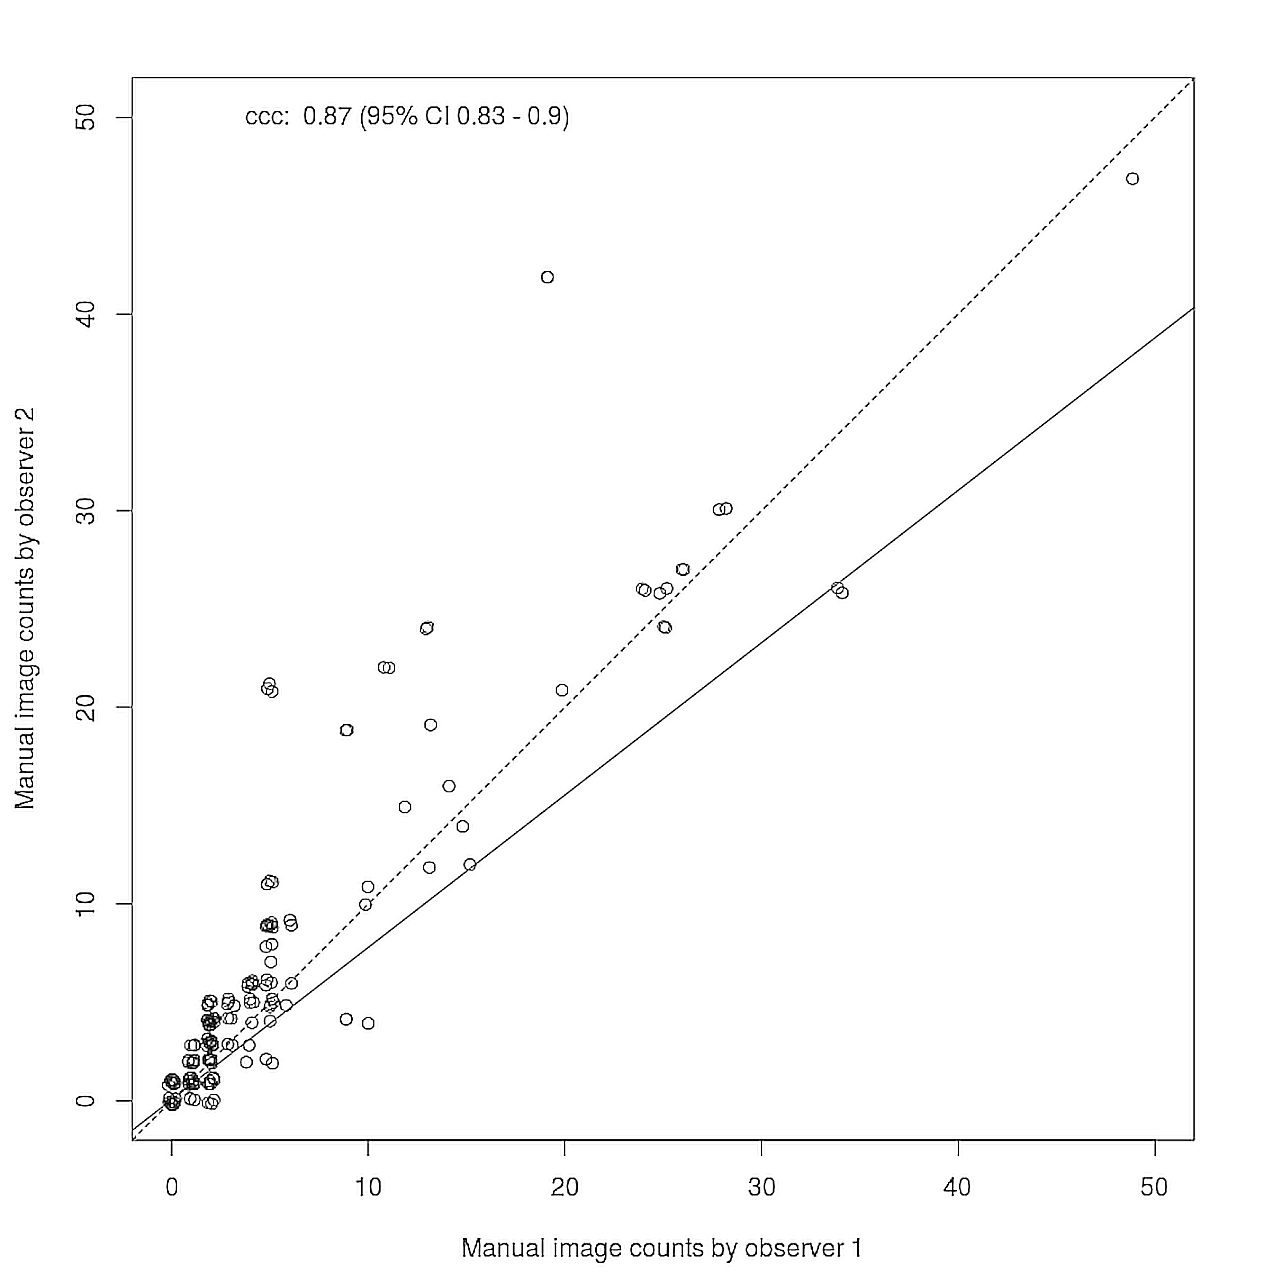
\includegraphics[width=1\linewidth]{gfx6/results/a2} \\
\caption[Manual counts by two scorers.]{Analysis 2: A comparison of nest counts estimated from images by different scorers (observer 1 and 2) image analysis methods. The dashed line shows perfect concordance; the solid line is the line of best fit. Performance measures: $r = 0.891$, $\rho_{c} = 0.867$ and $C_{b} = 0.973$.}\label{fig:manual-image-ob1-ob2-alldata}
\end{figure}

\begin{figure}[!htbp]\myfloatalign
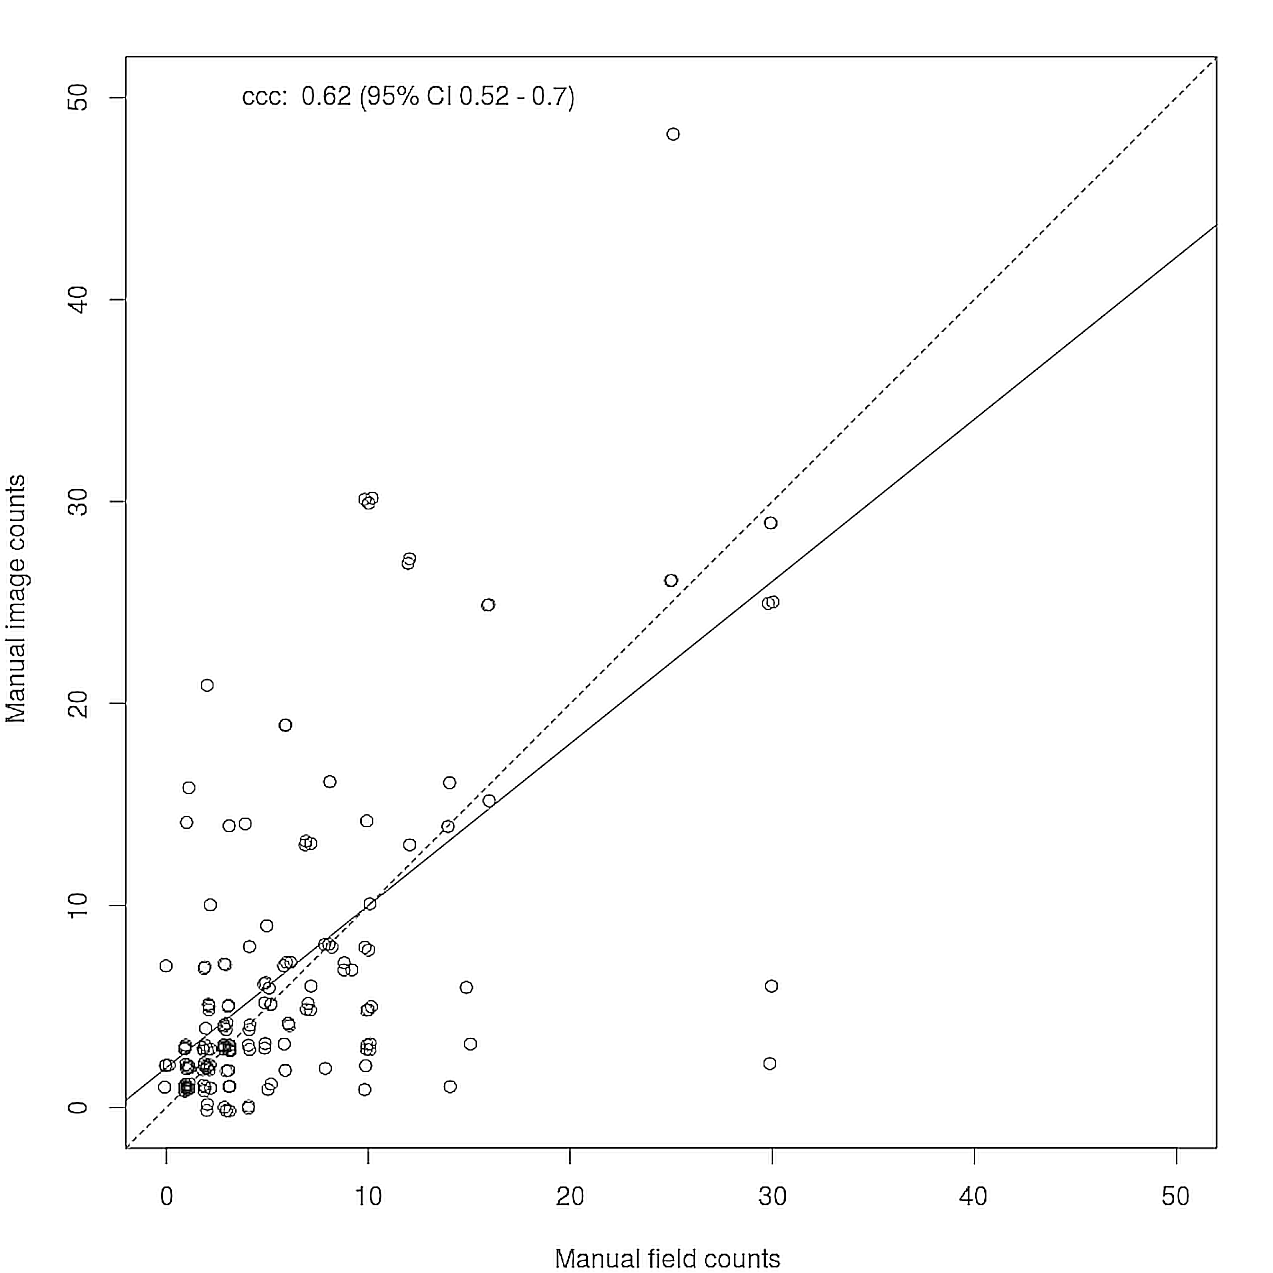
\includegraphics[width=1\linewidth]{gfx6/results/a3} \\
\caption[Manual image and field counts.]{Analysis 3: A comparison of manual-field and manual-image (mean counts from two observers $ n=170 $) nest counts. The dashed line shows perfect concordance; the solid line is the line of best fit. Performance measures: $r =  0.641$, $\rho_{c} = 0.622$ and $C_{b} = 0.97$.} \label{fig:manual-feild-manual-image}
\end{figure}

\subsection{Automatic and manual counts}\label{sec:automatic-and-manual-counts}
A comparison of nests counts estimated from images (the mean from two scorers $ n=170 $) and automatic counts derived from segmentations using the CF model are shown in Figure \ref{fig:manual-image-automatic-c4}. Manual-field  counts were compared to automatic counts derived using the CF model and are shown in Figure \ref{fig:manual-image-automatic-c4}. There was closer agreement between manual-field and automated-CF counts ($\rho_{c} = 0.738$), compared to manual-image counts ($\rho_{c} = 0.679$). The manual-field and manual-image counts  were slightly more accurate ($C_{b} = 0.963$) than automatic-CF counts ($C_{b} = 0.891$); both had similar precision (manual-image: $r = 0.705$, manual-field: $\rho_{c} =  0.738$).


\begin{figure}[!htbp]\myfloatalign
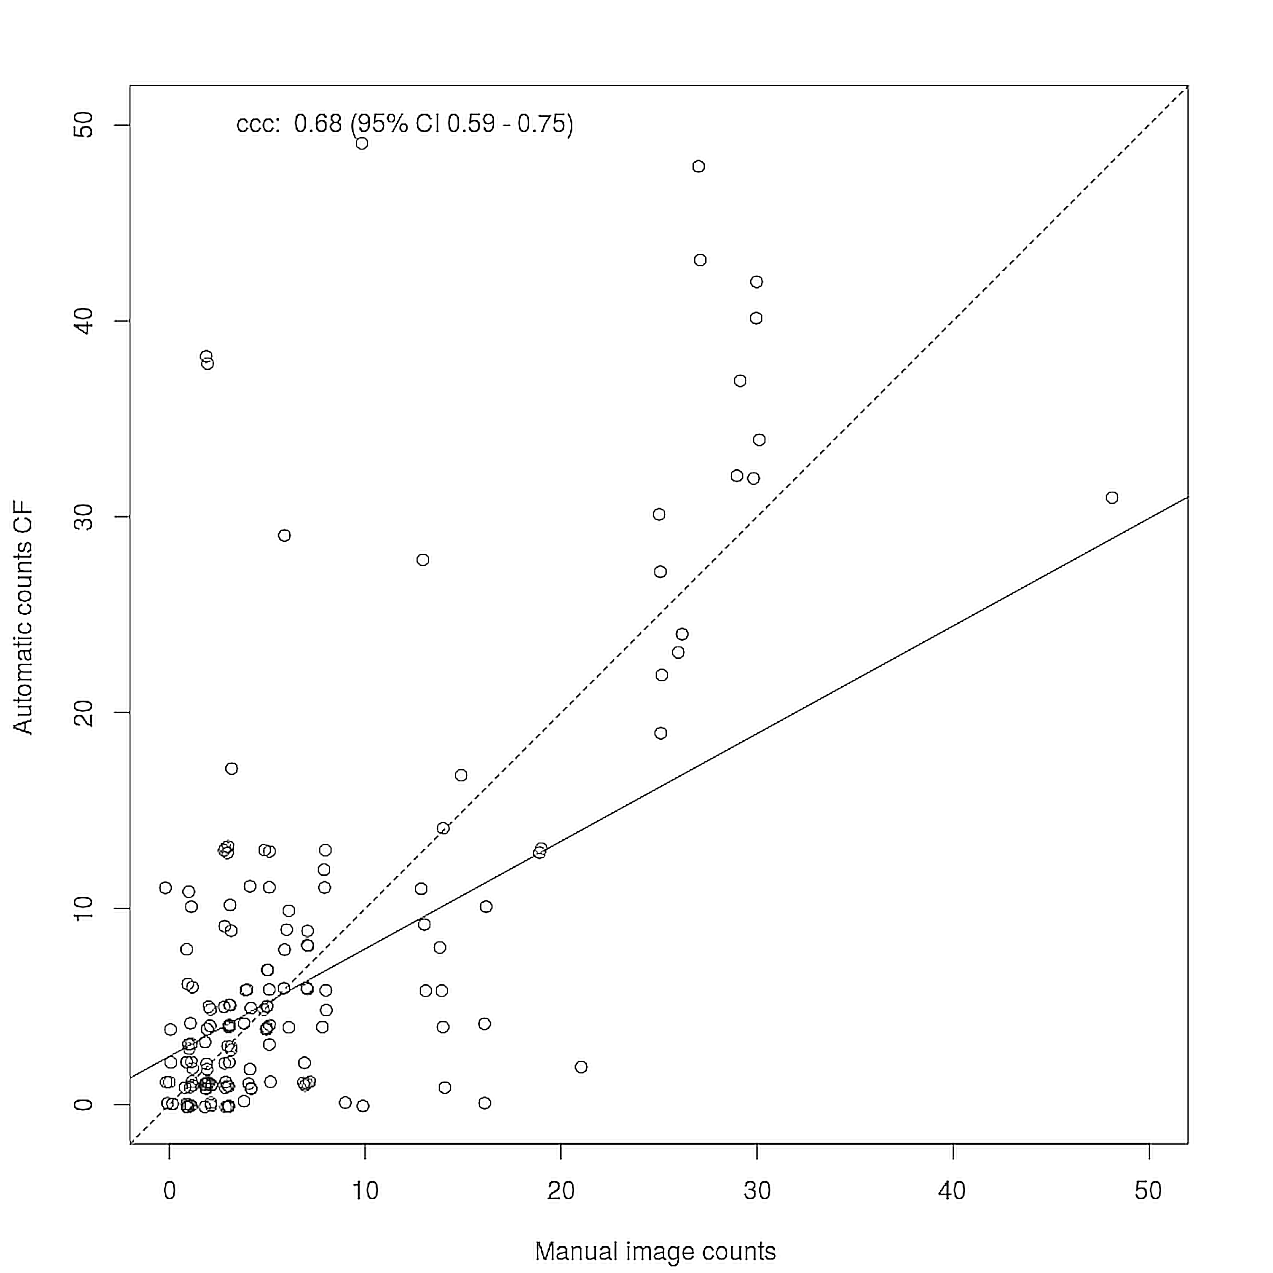
\includegraphics[width=1\linewidth]{gfx6/results/a4} \\
\caption[Manual image and automatic counts.]{Analysis 4: A comparison of manual-image nests counts (the mean from two scorers $ n=170 $) and automatic counts derived from the CF model. The dashed line shows perfect concordance; the solid line is the line of best fit. Performance measures: $r = 0.705$, $\rho_{c} = 0.679$  and $C_{b} = 0.963$.}  \label{fig:manual-image-automatic-c4}
\end{figure}

\begin{figure}[!htbp]\myfloatalign
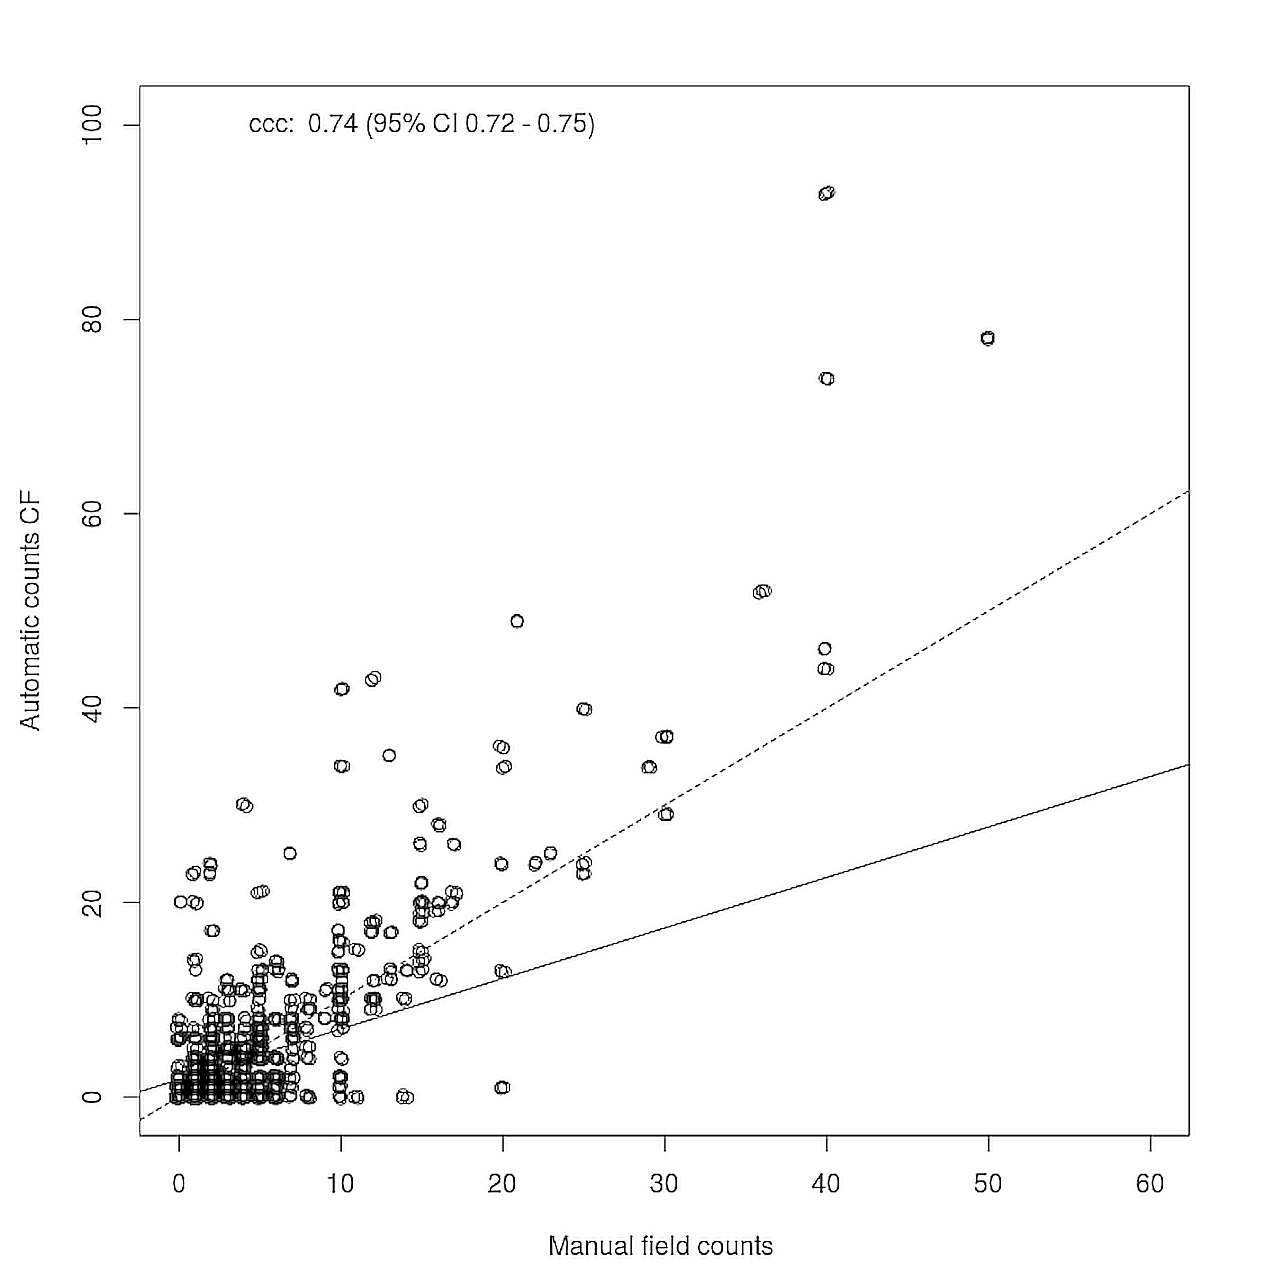
\includegraphics[width=1\linewidth]{gfx6/results/a5} \\
\caption[Manual field and automatic counts.]{Analysis 5: A comparison of manual-field and automatic nest counts derived from segmentations using the CF model (median of three image collections $n=520$). The dashed line shows perfect concordance;  the solid line is the line of best fit. Performance measures: $r = 0.828$, $\rho_{c} =  0.738$ and $C_{b} = 0.891$} \label{fig:manual-feild-automatic-c4}
\end{figure}

\clearpage

\section{Number of active nests by site and year}\label{sec:number-of-active-nests-by-site and year}
The number of active nests counted by three methods at each location are organised by year in Figures \ref{fig:changebysite1}, \ref{fig:changebysite2} and \ref{fig:changebysite3}. The changes in the number of active nests over time can be generally visualised for each site.  Methods produced similar temporal trends. Yearly mean values include error bars showing the standard error of the mean. Increased errors are associated with the number of monitoring samples collected ($n$) since they varied between sites and over time. Different methods produced more or less data samples (i.e. collections of near-replica images). For example, year 2014, $n=36$, from three monitoring days, three sites, four grids; if analysis used three image collections then $ n=108 $ (e.g. in the comparison of automatic counting methods).

\begin{table}[!htbp]\myfloatalign
\caption[Summary of monitoring samples.]{Number of yearly monitoring samples taken by the total number of monitoring days ($ n_{m} $), for three sites (S1, S2 and S3) and four grids. In 2014 $ n_{m} = 3 $ so the total number of samples for analysis used in manual field counts is $12$: $ n_{S1} = 12$ (site 1), $ n_{S2} = 12$ (site 2) and $ n_{S3} = 12$ (site 3).}\label{tab:summary-of-monitoring-samples}
\begin{tabular}{p{.6in}p{.6in}|p{.6in}p{.6in}p{.6in}} \toprule
 &	 & Samples &	 & \\
Year &	Method &	$ n_{S1} $ &	$ n_{S3} $ &	$ n_{S3} $ \\ \midrule
2010 &	ac &	126 &	130 &	 \\
 &	mic &	14 &	13 &	  \\
 &	mfc &	64 &	64 &		\\
2011 &	ac &	112 &	115 &	89  \\
 &	mic &	13 &	14 &	12 	 \\
 &	mfc &	64 &	64 &	64  \\
2012 &	ac &	114 &	116 &	74 \\
 &	mic &	13 &	21 &	5 	\\
 &	mfc &	52 &	52 &	52  \\
2013 &	ac &	105 &	105 &	90 \\
 &	mic &	17 &	14 &	8 	 \\
 &	mfc &	40 &	40 &	40 \\
2014 &	ac &	36 &	36 &	36  \\
 &	mic &	10 &	7 &	7  \\
 &	mfc &	12 &	12 &	12  \\
$ n_{ac} = $ & 1284	 &	 &	 &	 	 \\
$ n_{mic} = $ & 170	 &	 &	 &	 	 \\
$ n_{mfc} = $ &	632 &	 &	 &	 	 \\
\bottomrule
\end{tabular}
\end{table}

\subsection{Mt. Tiger}\label{sec:mt.-tiger}
The trends in active nests from data collected  over five years (2010--2014) on Mt. Tiger are shown in Figure \ref{fig:changebysite1} below. There was a sharp decline in the mean number of active nests between 2010 and 2011; little changes between 2011 to 2013, with an increase in the mean number of active nests in 2014 ($n_{S1} = 12$). Similar trends were displayed by all methods. The automatic counts derived from image segmentation using the CF model (red), on average produced slightly higher mean counts than manual image (green) and manual field counts (blue).

\begin{sidewaysfigure}[!htbp]\myfloatalign
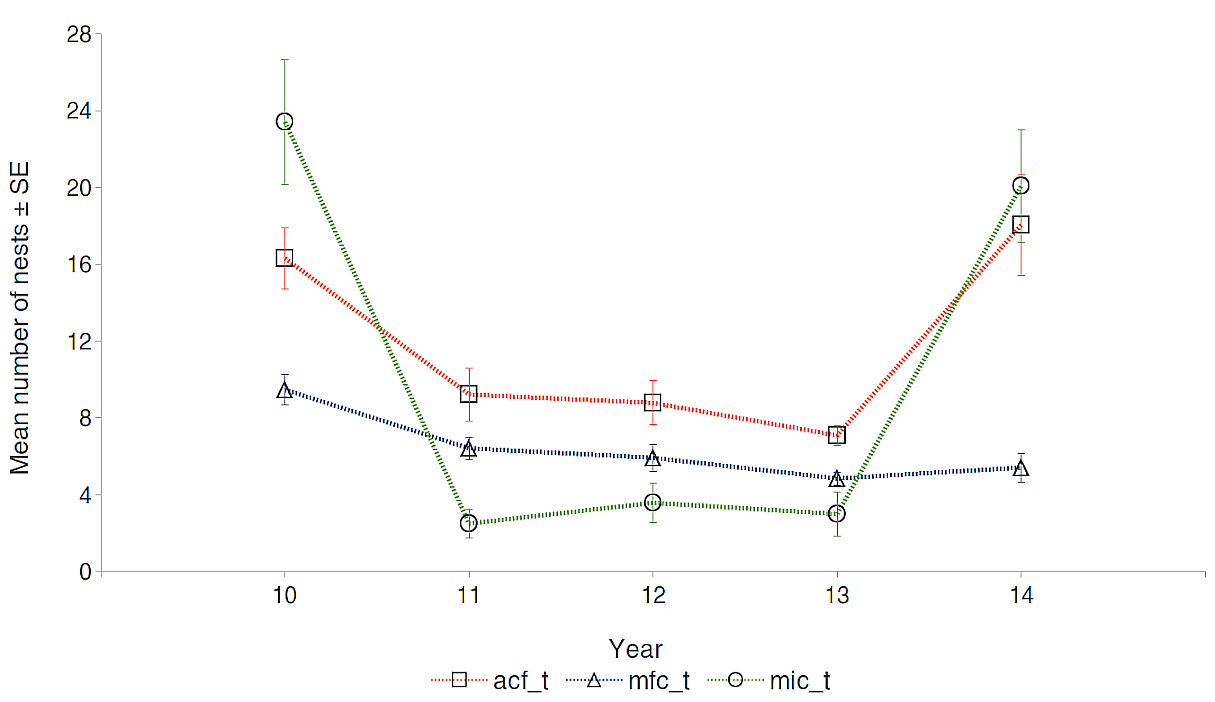
\includegraphics[width=0.9\linewidth]{gfx6/change/changebysite1} \\
\caption[Yearly nest counts site 1.]{Site 1:  Yearly mean  nest counts \textpm $ SE$ (error bars) by three methods. Automatically derived segmentations from CF model - $ act\_t, n = 493 $, manual field counts (red) - $ mfc\_t, n = 232 $ (blue) and manual image counts - $ mic\_t, n = 67 $ (green).}\label{fig:changebysite1}
\end{sidewaysfigure}

\subsection{Mt. Parihaka}\label{sec:mt.-parihaka}
The trends in active nests from data collected  over five years (2010--2014) on Mt. Parihaka are shown in Figure \ref{fig:changebysite2} below. There was a moderate decline in the mean number of active nests between 2010 and 2012; and a gradual increase the mean number of active nests recorded in 2012 and 2014. Similar trends were displayed by all methods. The automatic counts derived from image segmentation using the CF model (red), on average produced slightly higher mean counts than manual image counts (blue) but lower than manual field counts (green).

\begin{sidewaysfigure}[!htbp]\myfloatalign
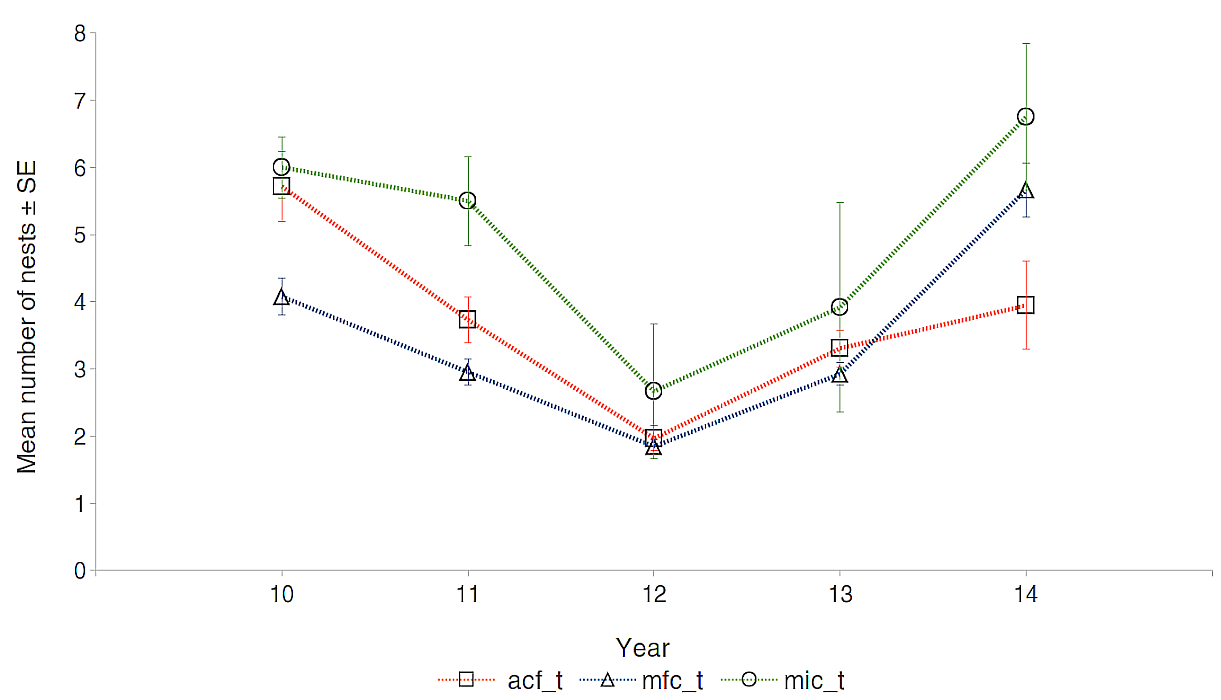
\includegraphics[width=.9\linewidth]{gfx6/change/changebysite2} \\
\caption[Yearly nest counts site 2. ]{Site 2:  Yearly mean  nest counts  \textpm $SE$ (error bars) by three methods. Automatically derived segmentations from CF model - $ act\_t, n = 502 $ (red), manual field counts - $ mfc\_t, n = 232 $ (blue) and manual image counts - $ mic\_t, n = 69 $ (green).}\label{fig:changebysite2}
\end{sidewaysfigure}

\subsection{Memorial Drive}\label{sec:memorial-drive}
The trends in active nests from data collected  over four years (2011--2014) on Memorial Drive  are shown in Figure \ref{fig:changebysite3} below. There was a moderate decline in the mean number of active nests between 2011 and 2013; and a gradual increase the mean number of active nests recorded in 2014. Similar trends were displayed by all methods. The automatic counts derived from image segmentation using the CF model (red), on average produced slightly lower mean counts than manual image (blue) and manual field counts (green).

\begin{sidewaysfigure}[!htbp]\myfloatalign
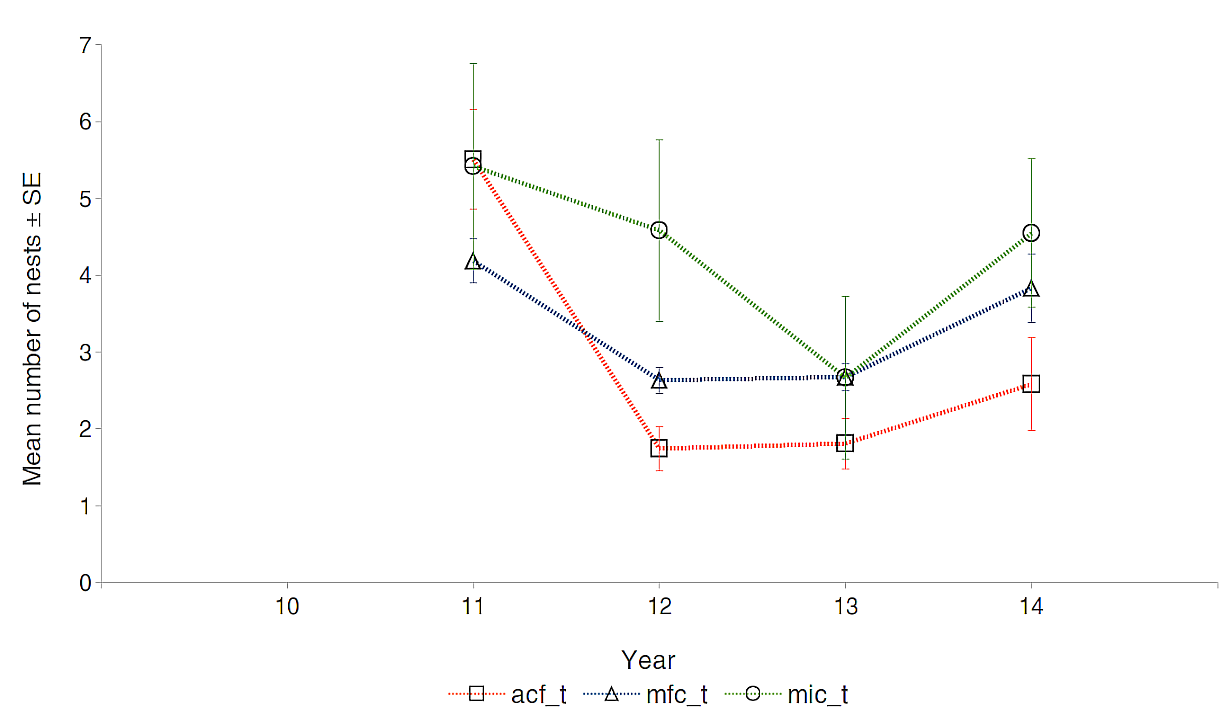
\includegraphics[width=0.9\linewidth]{gfx6/change/changebysite3} \\
\caption[Yearly nest counts site 3.]{Site 3:  Yearly mean nest counts \textpm $SE$ (error bars) by three methods. Automatically derived segmentations from CF model - $ act\_t, n = 289 $ (red), manual field counts - $ mfc\_t, n = 168 $ (blue) and manual image counts - $ mic\_t, n = 34 $ (green).}\label{fig:changebysite3}
\end{sidewaysfigure}
\clearpage

